\documentclass[conference]{IEEEtran}
\IEEEoverridecommandlockouts
% The preceding line is only needed to identify funding in the first footnote. If that is unneeded, please comment it out.
\usepackage{cite}
\usepackage{amsmath,amssymb,amsfonts}
\usepackage{algorithmic}
\usepackage{graphicx}
\usepackage{textcomp}
\usepackage{xcolor}
\def\BibTeX{{\rm B\kern-.05em{\sc i\kern-.025em b}\kern-.08em
    T\kern-.1667em\lower.7ex\hbox{E}\kern-.125emX}}
\begin{document}

\title{Steam Store Games Exploratory Data Analysis\\}

\author{\IEEEauthorblockA{Hazar Belge}
Galatasaray University, Computer Engineering\\
Istanbul, Turkey \\
Introduction to Data Analysis}

}

\maketitle


\section{Introduction}
	Steam is a video game digital distribution service by Valve. It was launched as a standalone software client in 2003 as a way for Valve to provide automatic updates for their games and expanded to include games from third-party publishers. Steam has also expanded into an online web-based and mobile digital storefront. 

	In this paper, we will look into a dataset about different video games with their different attributes like price, owner count, playtime, achievements count etc.

	After describing the parameters and data in a comprehensive manner, we will ask a high-level research question and a low-level technical questions. Finally, we will have a description of the methods we intend to use to answer these questions.

\section{Steam Dataset}
This dataset is published by Nik Davis on Kaggle. It includes 27075 different video games and 18 different attributes for each of them from Steam. The dataset was last updated in May 2019, so I removed the games that were released in 2019 to prevent them from misleading the year-to-year comparison. After this removing process we have 24862 video games in total. So, let's take a look at some of attributes of dataset.

\subsection{Achievements}
Achievements are designed to increase a player's enjoyment of the video game and elicit a sense of satisfaction. When we think about it in this context, can we say that every developer company who tries to be successful has put achievements in its game? Let's see what the situation is. 

\begin{figure}[ht]
  \centering
  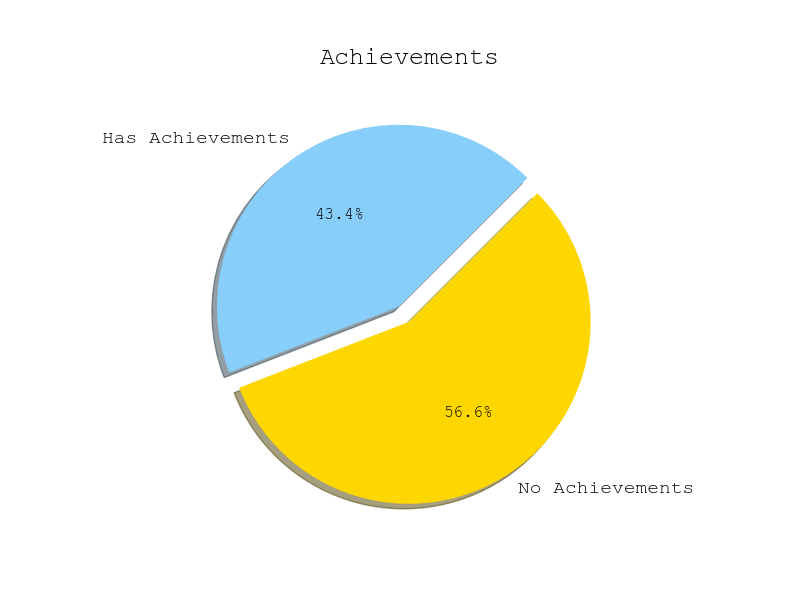
\includegraphics[width=6cm,height=6cm,keepaspectratio]{assets-1/achievements_pie.png}
  \caption{How many games have achievements?}
  \label{fig:achievements1}
\end{figure}

As we can see from Fig. 1., although the majority of video games prefer to put achievements in their games, the rate of those who do not (43.4\%) is not low.

\begin{figure}[ht]
  \centering
  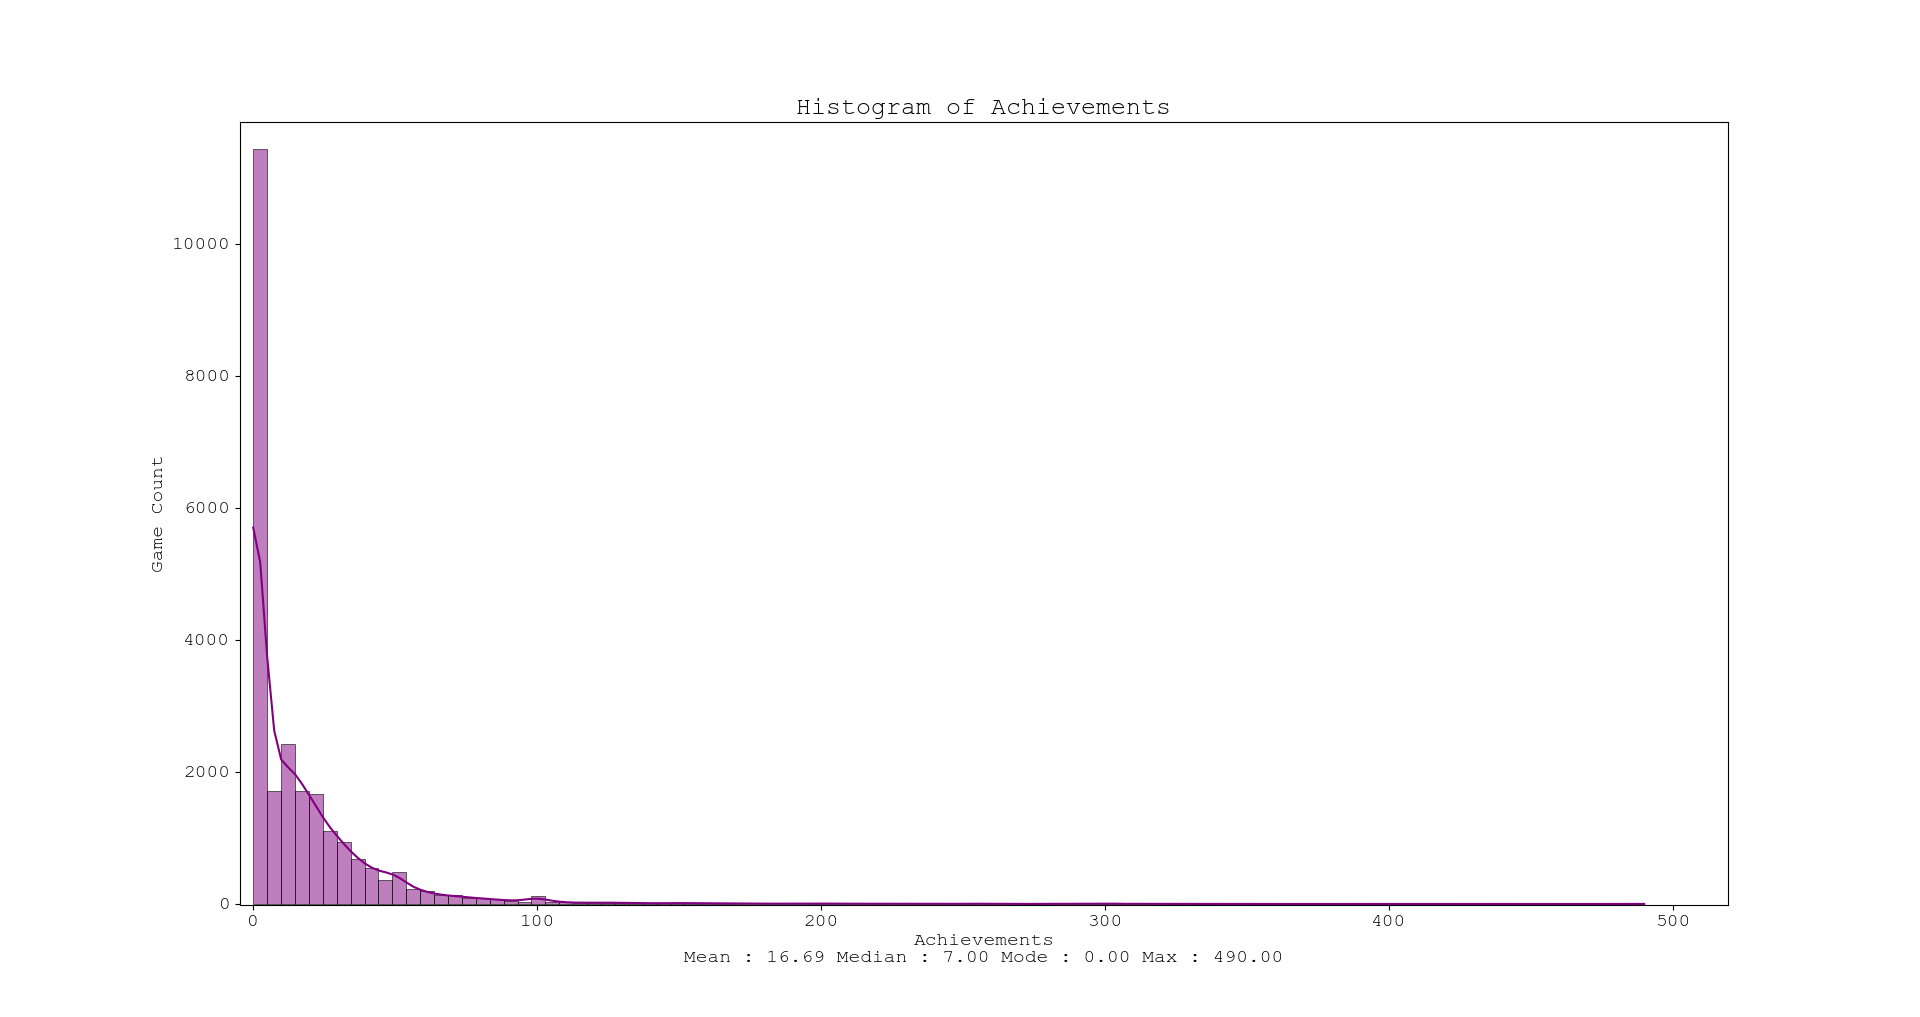
\includegraphics[width=\linewidth]{assets-1/achievements_hist.png}
  \caption{Histogram of Achievements.}
  \label{fig:achievements2}
\end{figure}

When we look at Fig. 2., we can easily see that video games do not want to increase the number of achievements. As the number of achievements decreases, the number of games belonging to that achievement number increases.

\subsection{Age Rating}
Age Rating is a somewhat complex/indirect feature. Video games do not directly choose their age rating. The combination of genre, subject  and content of the video games that they created makes that age restriction necessary. That's why developers have 3 options. Reducing adult content and lowering or resetting the age limit. Not reducing adult content and ignoring the high age limit. Those who try to find a way by lowering the adult content and age restriction by a certain degree.

\begin{figure}[ht]
  \centering
  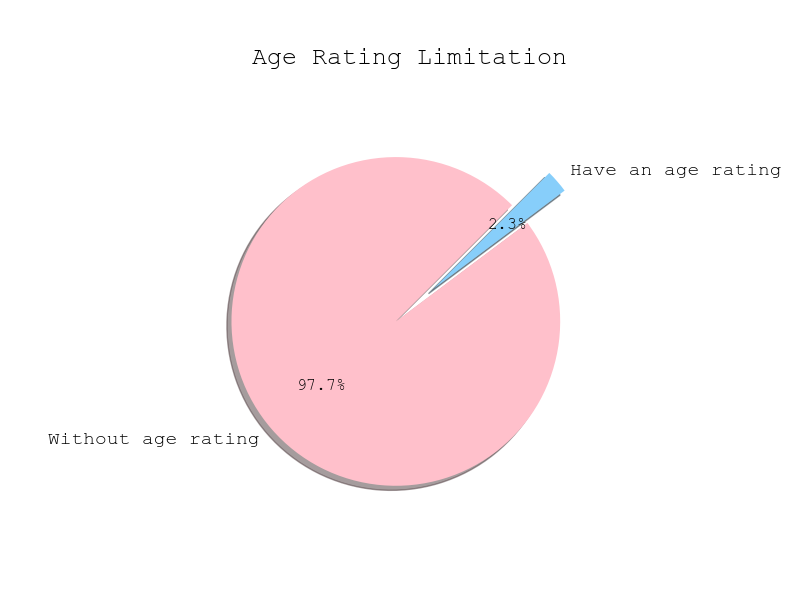
\includegraphics[width=6.25cm,height=6.25cm,keepaspectratio]{assets-1/age_rating_pie.png}
  \caption{How many games have age rating?}
  \label{fig:agerating1}
\end{figure}

We can clearly see that the vast majority did not choose to use age-restricted content in their games (Fig. 3.).

\begin{figure}[ht]
  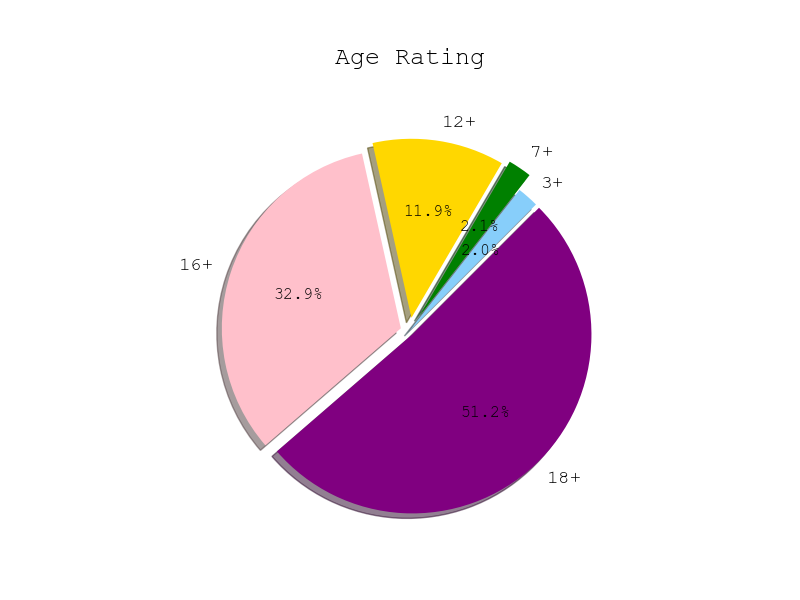
\includegraphics[width=\linewidth]{assets-1/age_rating_has_pie.png}
  \caption{Age Ratings Pie Chart.}
  \label{fig:agerating2}
\end{figure}

However, we can say that those who choose to use adult content prefer to have more or high-level content and do not care about the age limit (Fig. 4.). 

\subsection{Category}
\begin{figure}[h]
  \centering
  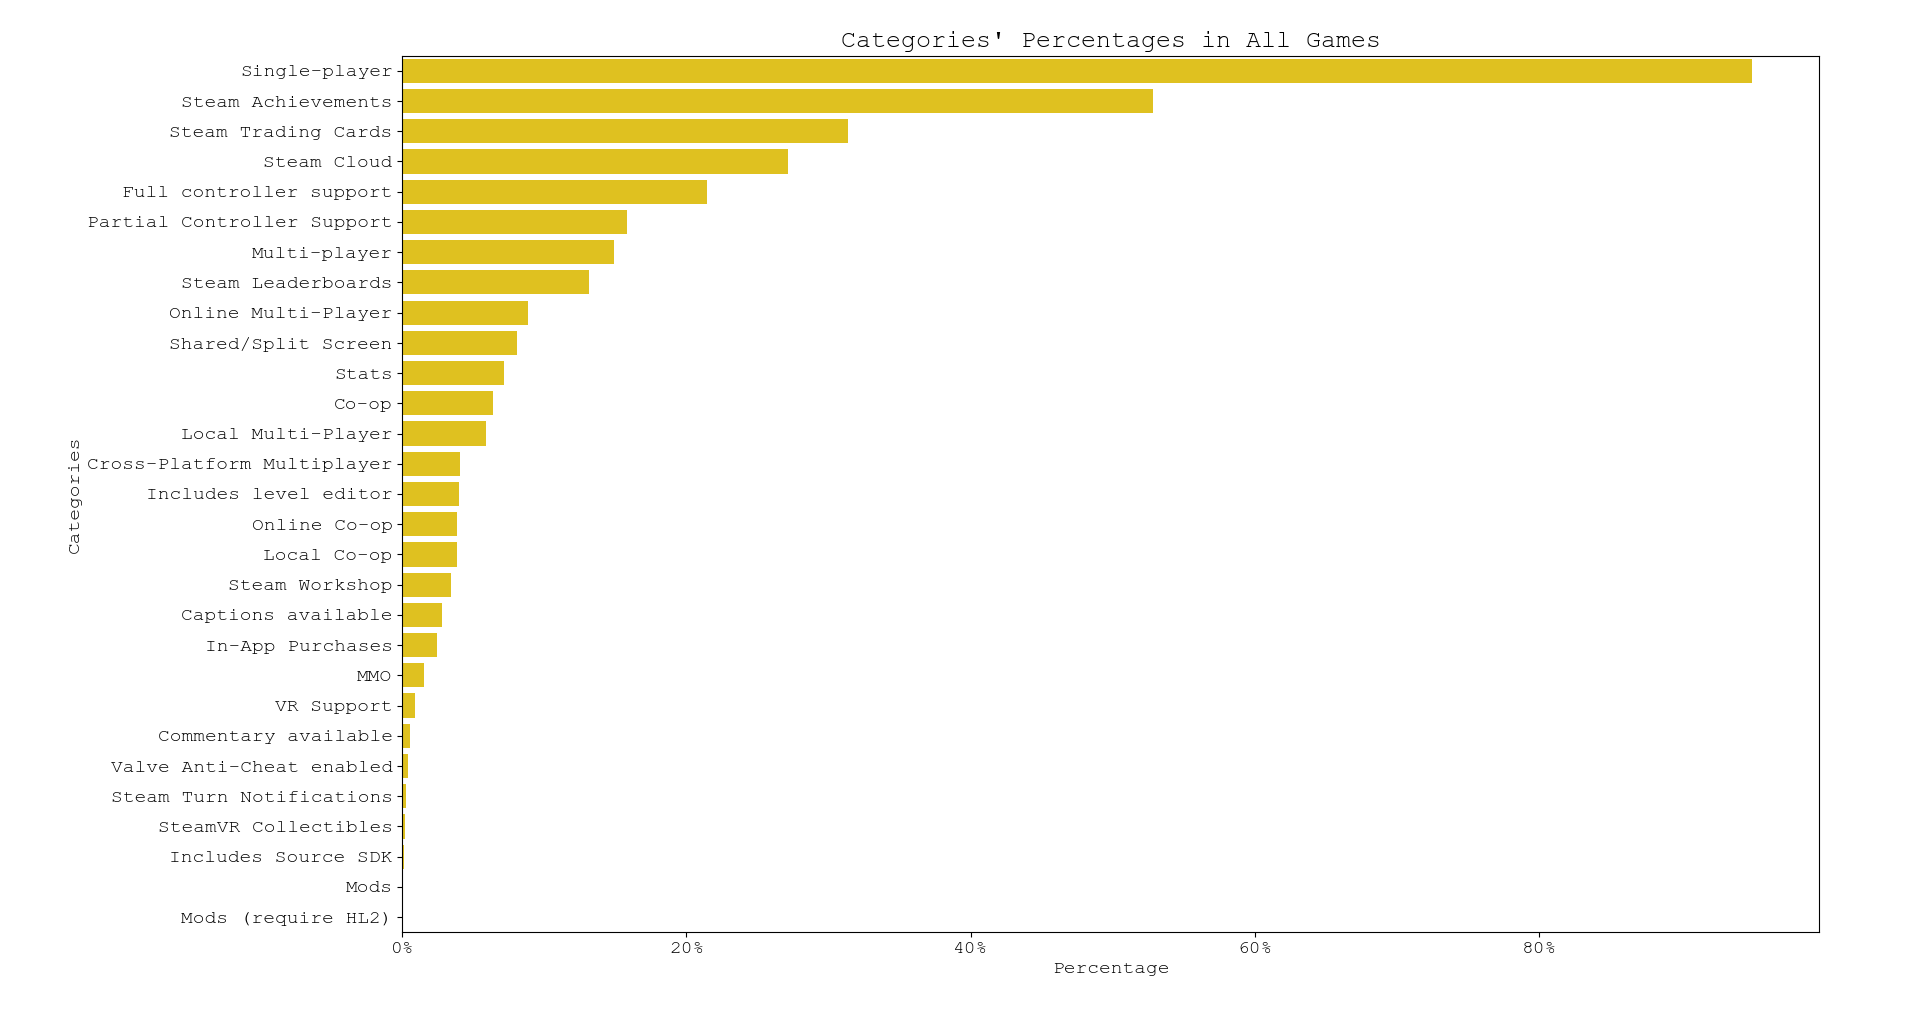
\includegraphics[width=\linewidth,height=7.9cm]{assets-1/categories_dist.png}
  \caption{Categories' percentages of all games.}
  \label{fig:category1}
\end{figure}

Fig.5. shows us that the majority of video games are in the single-player category. While multi-player games are in the minority, the single-player category is followed by games with achievements and games where you can win and trade cards.

\subsection{English Support}

Supporting the English language, which is the most spoken language in the world, also plays a big role in increasing the number of people you can reach. 

\begin{figure}[ht]
  \centering
  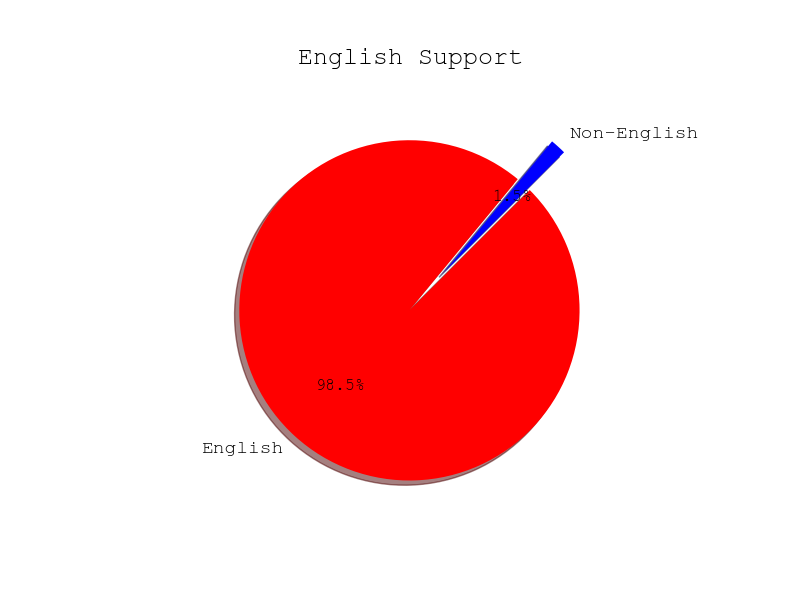
\includegraphics[width=\linewidth]{assets-1/english_support_pie.png}
  \caption{How many games have English support?}
  \label{fig:englishsupport1}
\end{figure}

Fig. 6. shows us that 98.5\% of 24862 video games, or 24489, support the English language.

\subsection{Genre}


\begin{figure}[h]
  \centering
  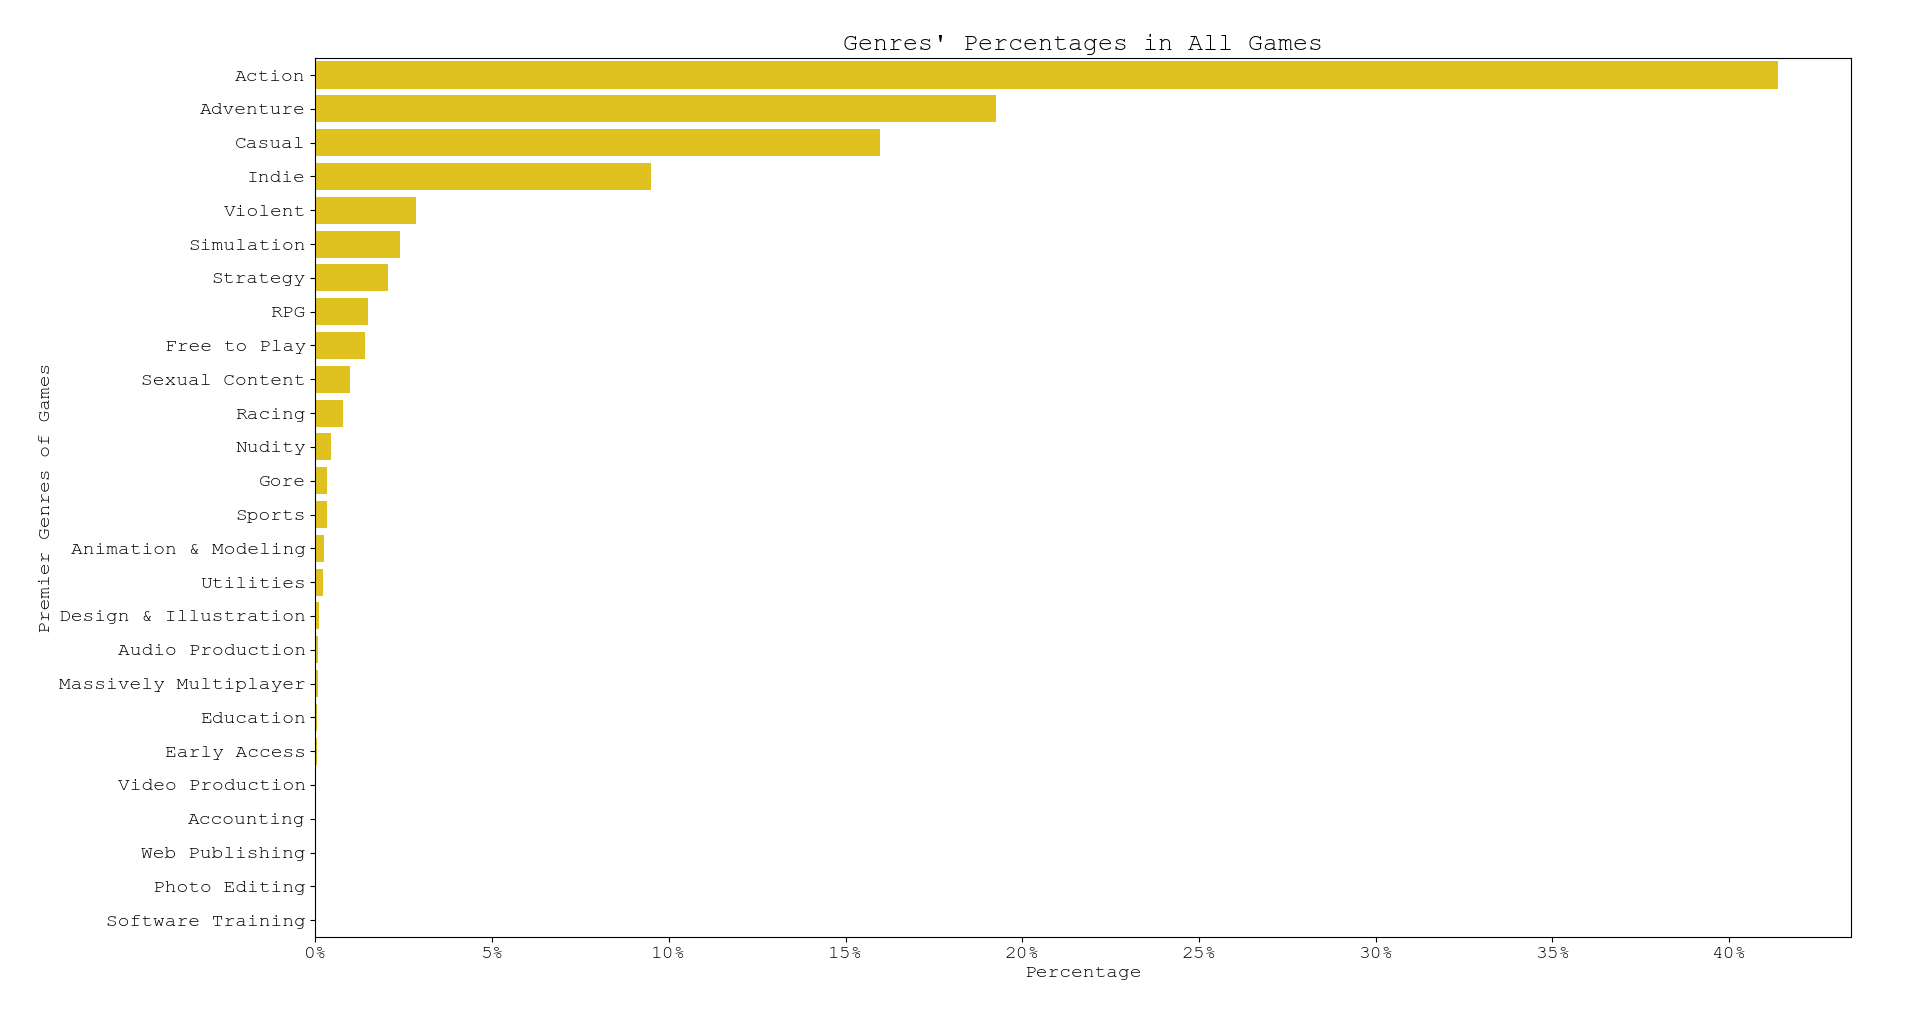
\includegraphics[width=\linewidth,height=7.9cm]{assets-1/genres_dist.png}
  \caption{Genres' percentages of all games.}
  \label{fig:genre1}
\end{figure}

Fig. 7. shows us that the majority of video games are in the action genre. The action genre is followed by adventure, casual, indie and violent games, respectively. \\

\subsection{Owner Count}
Owner Count is the main attribute of the steam dataset. Naturally, we can easily predict that as the owner count increases, the number of video games belonging to that count will decrease. In this exploratory data analysis, we examine why video games that reach 2M+ owners and 1M-2M owners sell this much.

\begin{figure}[h]
  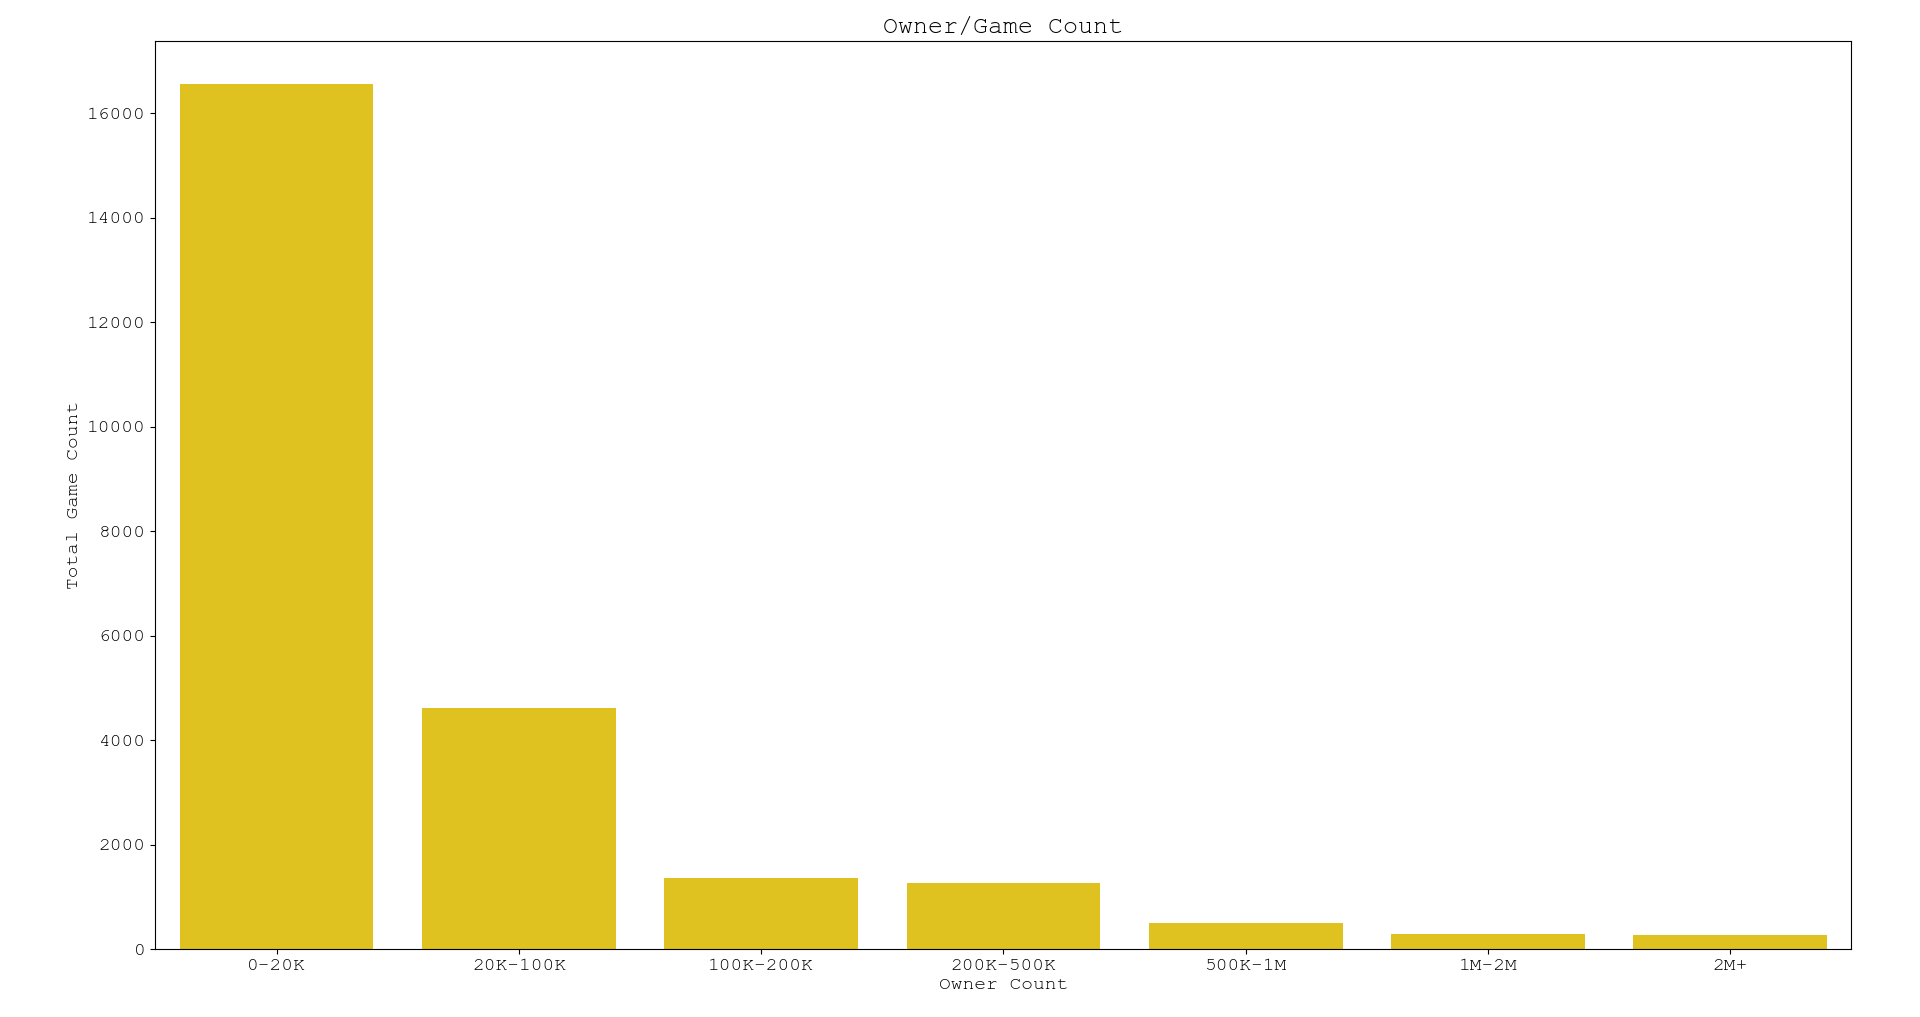
\includegraphics[width=\linewidth, height=6cm]{assets-1/owners_count.png}
  \caption{Distribution of owners count in all games.}
  \label{fig:ownercount1}
\end{figure}


\subsection{Platform}
The platform on which the video game will be played is very important. While it is known that Windows-supporting machines are the majority today, developing games only for Mac or Linux is a project that will fail as a result. In addition, developing games only for Windows and leaving Mac or Linux users out will cause loss of users up to a certain level, although not as much as the opposite.

\begin{figure}[h]
  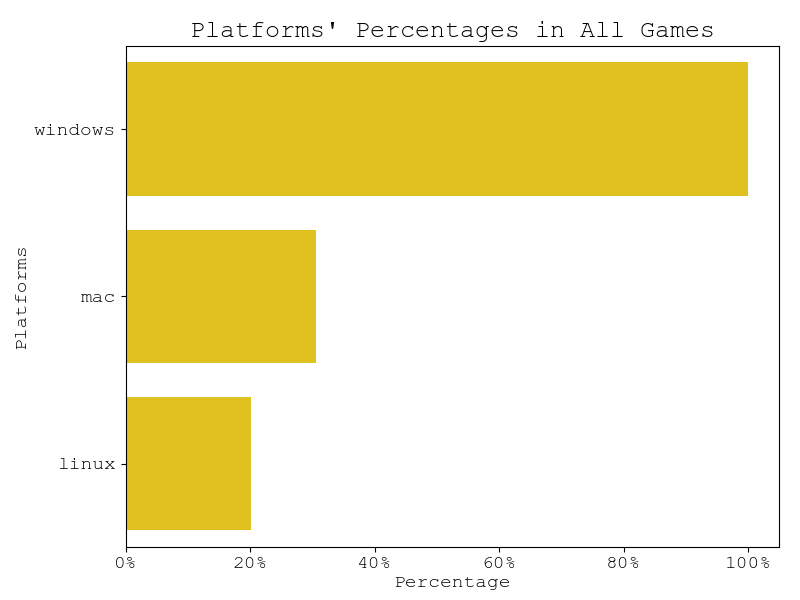
\includegraphics[width=\linewidth, height=5cm]{assets-1/platforms_dist.png}
  \caption{Platforms' percentages of all games.}
  \label{fig:platform1}
\end{figure}

As we can easily see from Figure 9, almost 100\% of 24862 video games support the Windows platform (99.97\%). The Windows platform is followed by Mac with 30.59\% and Linux with 20.07\%.

\subsection{Positive Rate}
The positive rate attribute was synthesized from the existing positive\_reviews and negative\_reviews columns in the dataset. It is a value between 0 and 1 obtained by dividing the number of positive reviews by the total number of reviews.

\begin{figure}[h]
  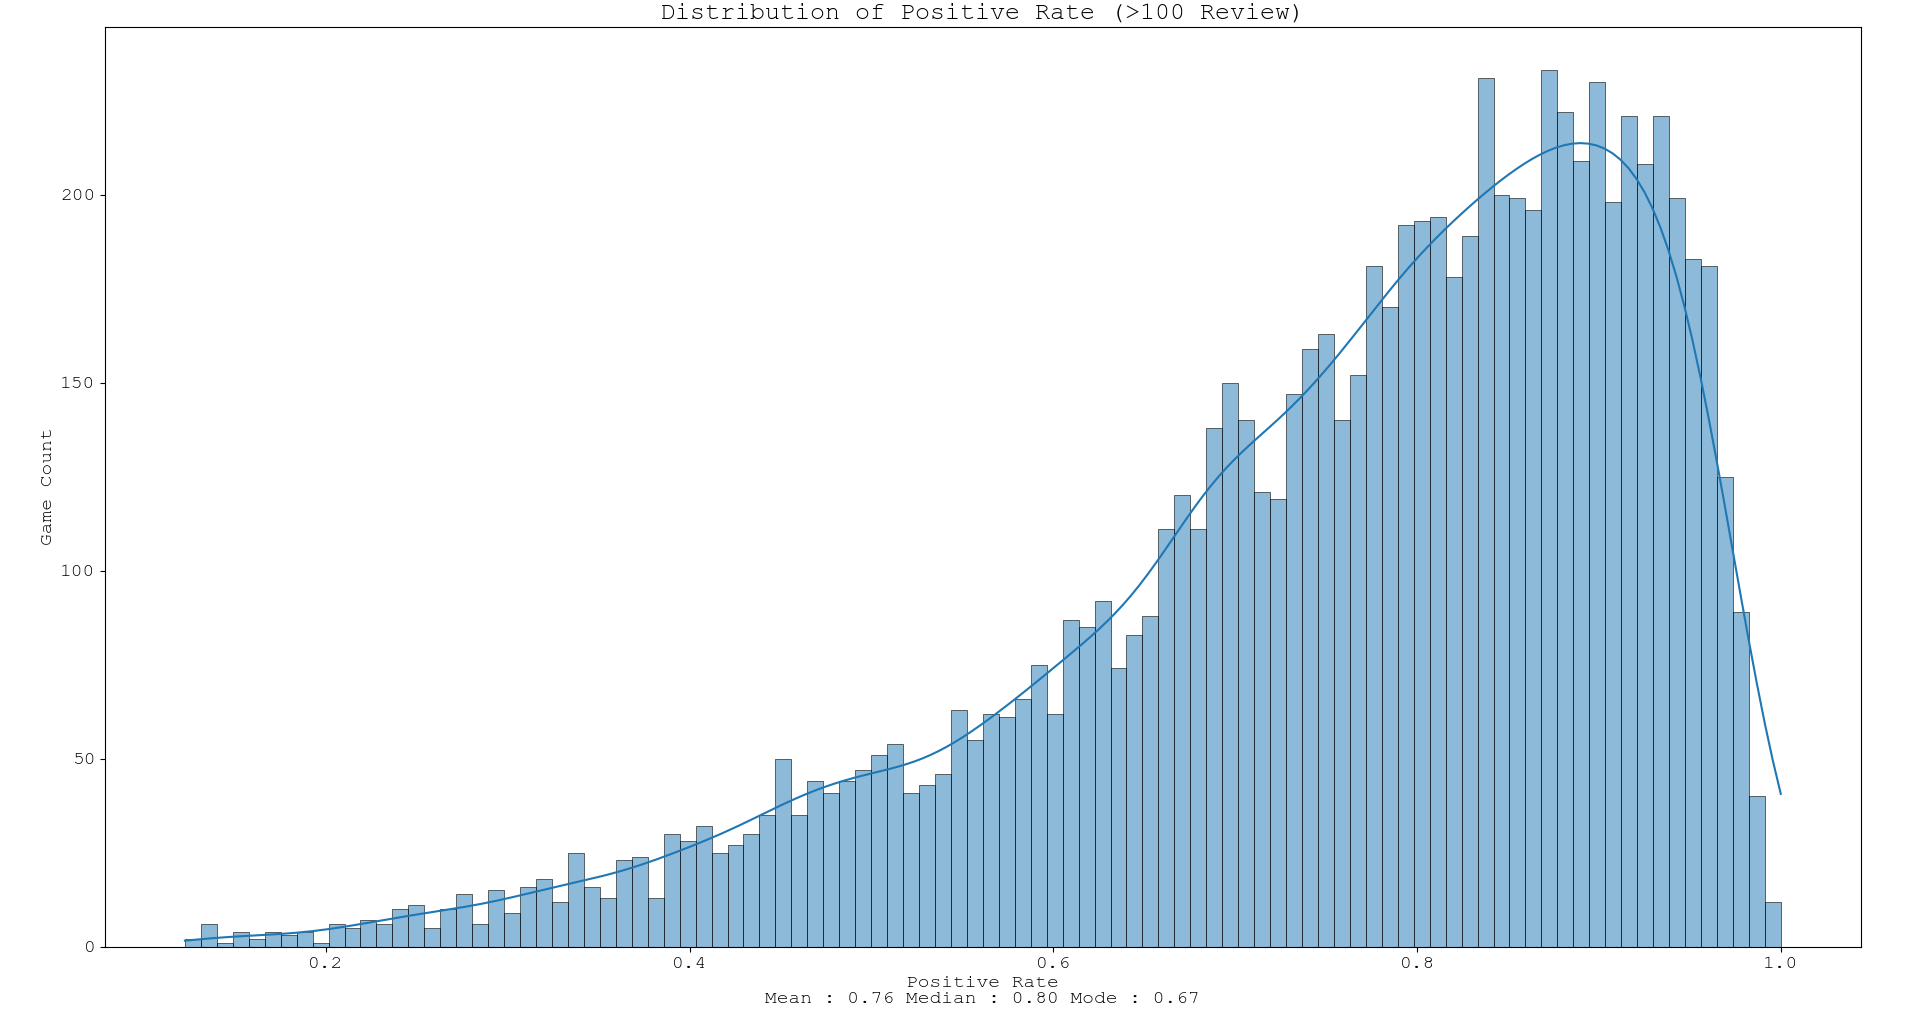
\includegraphics[width=\linewidth]{assets-1/positive_rate_dist.png}
  \caption{Histogram of Positive Rate.}
  \label{fig:positiverate1}
\end{figure}

The positive rate distribution is concentrated around 0.8, although it does not appear on the histogram due to the fact that bins=100 and a value between 0 and 1, its mode is equal to 0.6667, mean is 0.7583 and median is 0.7959. \\

\subsection{Price}
Perhaps the most important factor that comes to mind when it comes to game sales is price. While some developers try to make the game free to reach more people and generate income with microtransactions, other companies want to remove the costs directly from the sale.

\begin{figure}[h]
  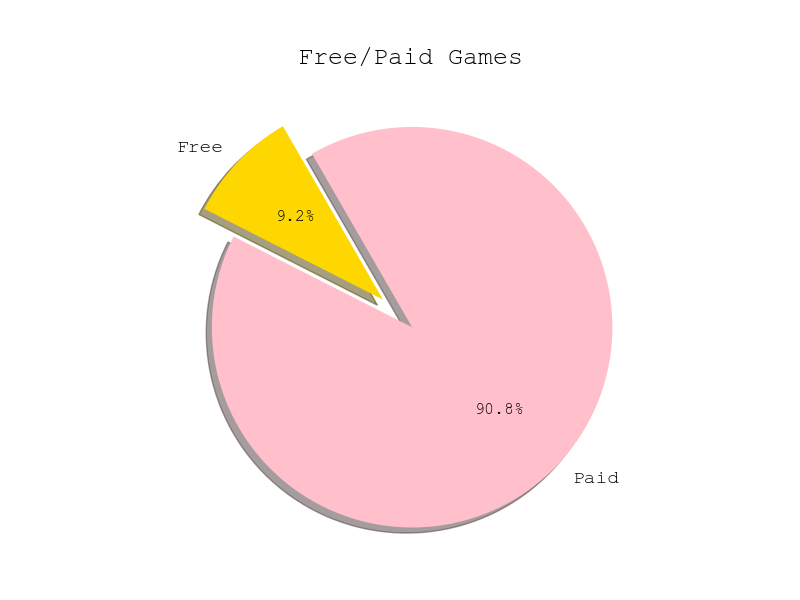
\includegraphics[width=\linewidth, height:5cm]{assets-1/price_free_paid_pie.png}
  \caption{How many games are paid?}
  \label{fig:price1}
\end{figure}

As we can see in Figure 11, the percentage of developers making the game free is only 9.2\%. \\\\

\begin{figure}[h]
  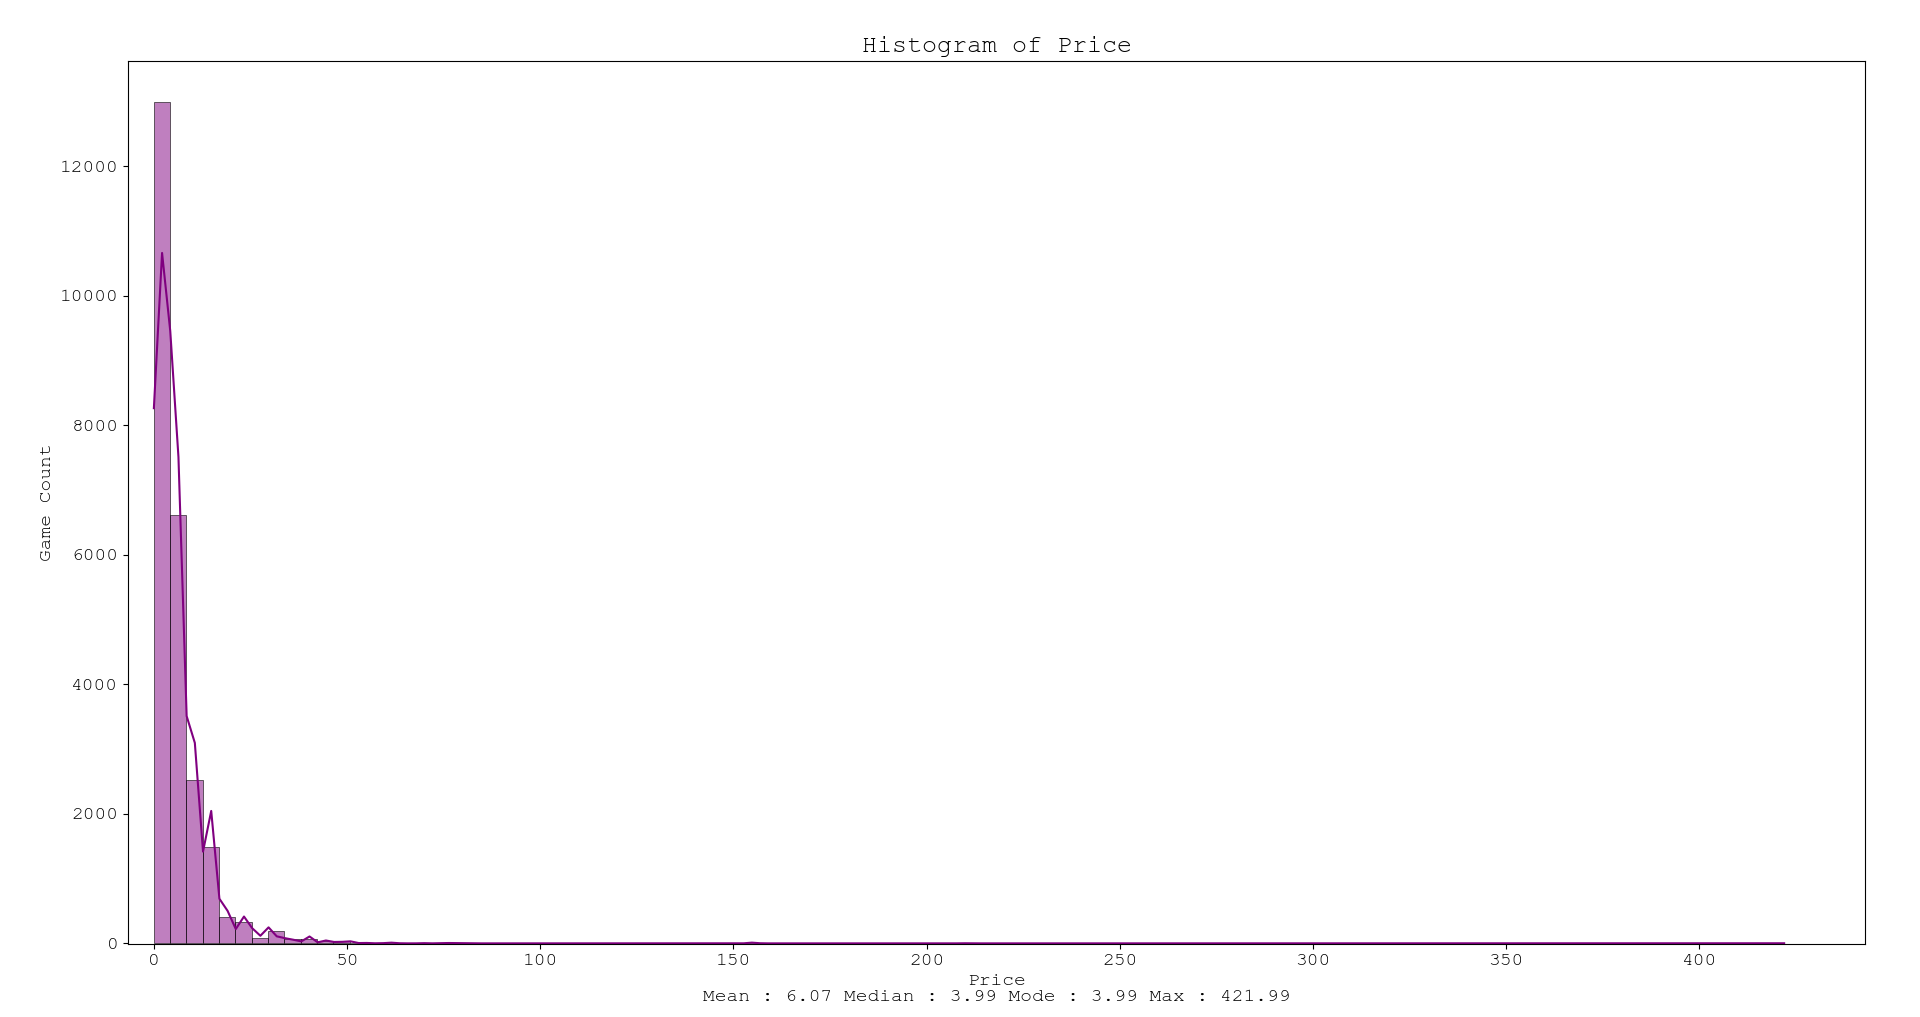
\includegraphics[width=\linewidth, height=6cm]{assets-1/price_hist.png}
  \caption{Histogram of Price.}
  \label{fig:price2}
\end{figure}

In the histogram that we can see in Figure 12, the majority of the games are between \$0 and \$50, but the video games that can be called Triple-A with the maximum value of \$421 have extended the histogram to the right in the x-axis.

\subsection{Released Date}


\begin{figure}[h]
  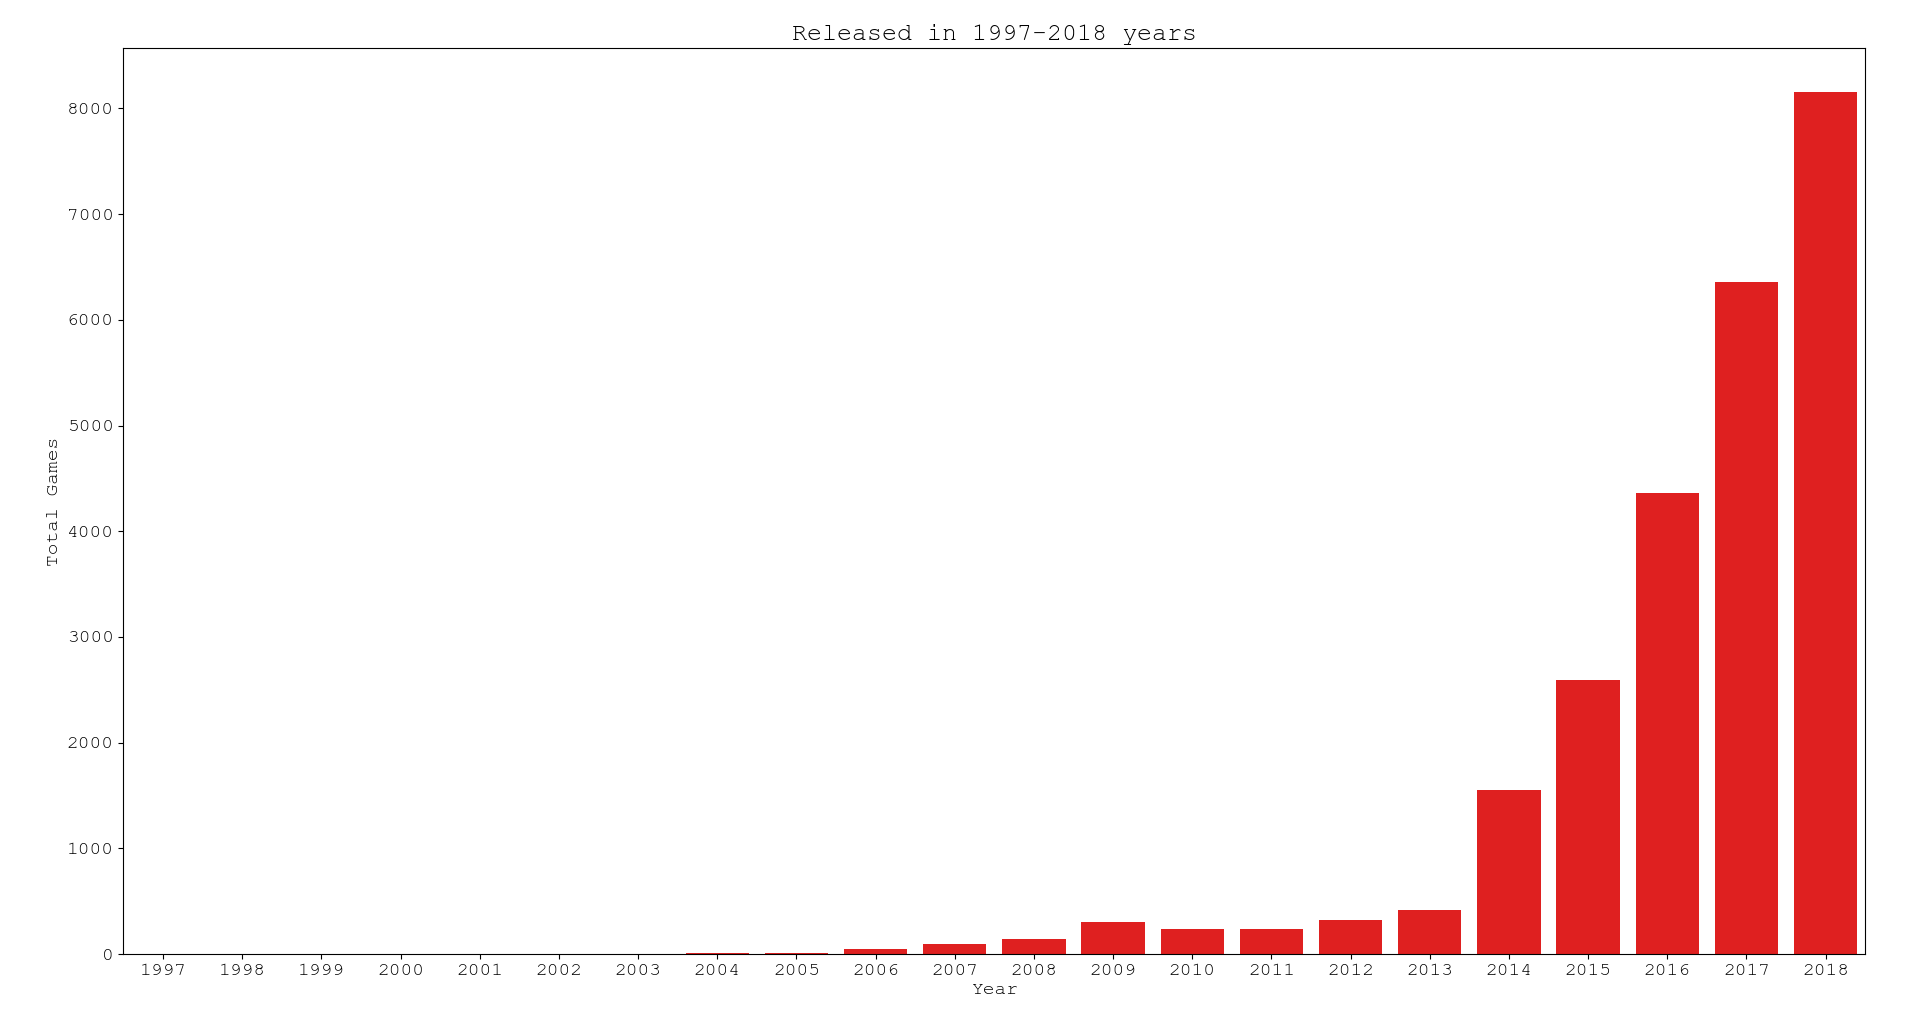
\includegraphics[width=\linewidth, height=5cm]{assets-1/released_date_bar.png}
  \caption{Video Games Per Year.}
  \label{fig:releaseddate1}
\end{figure}

From Figure 13, we can clearly see that the number of video games released every year is constantly increasing.

\section{Questions about the steam data}
We need the high-level research question to analyze the data and parameters. Then we need low-level technical questions to support this high-level question. With all these questions, we can reach the result more easily.

\subsection{The High Leve Research Question: What are the attributes that affect game sales the most?}\label{AA}
While developing video games, the sales numbers of the game and the income we can generate from it are very important. That's why we want our game to sell well, but it is not certain what are the attributes that make this sale big. There are many factors that will affect game sales. While Flappy Bird with almost no budget makes millions, the game with a budget of millions of dollars may not be liked at all and may not make a profit. Which brings us to our high-level research question that may reveal the solution to this problem. “What are the attributes that affect game sales the most? Of course, we also need subquestions to answer this question.

\subsection{Low Level Technical Questions}
\begin{itemize}
\item Does having more achievements affects the game sales positively?
\item Do higher age ratings affect the game sales negatively?
\item Does having english support affects the game sales positively?
\item Do genres affect the game sales?
\item Do categories affect the game sales?
\item Does developers' name affects the game sales?
\item Does having more platform support affects the game sales positively?
\item Do higher prices affect the game sales negatively?
\item Does publishers' name affects the game sales?
\item Do release dates affect the game sales?
\item Does having more reviews affects the game sales positively?
\end{itemize}


\section{Hypothesis Tests And The
Methods}

\subsection{Hypothesis Tests}

\begin{itemize}
    \item "Does having more achievements affects the game sales positively?" This question is about a relationship between two different data.\\Null
Hypothesis: There isn't any relation between achievements and owners count.\\ Alternative Hypothesis: There is a relation between achievements and owners count. \\
    \item "Do higher age ratings affect the game sales negatively?" This question is about a relationship between two different data.\\Null
Hypothesis: There isn't any relation between age ratings and owners count.\\ Alternative Hypothesis: There is a relation between age ratings and owners count. \\
    \item "Does having english support affects the game sales positively?" This question is about a relationship between two different data.\\Null
Hypothesis: There isn't any relation between having english support and owners count.\\ Alternative Hypothesis: There is a relation between having english support and owners count. \\
    \item "Do genres affect the game sales?" This question is about a relationship between two different data.\\Null
Hypothesis: There isn't any relation between genres and owners count.\\ Alternative Hypothesis: There is a relation between genres and owners count. \\
    \item "Do categories affect the game sales?" This question is about a relationship between two different data.\\Null
Hypothesis: There isn't any relation between categories and owners count.\\ Alternative Hypothesis: There is a relation between categories and owners count. \\
    \item "Does developers' name affects the game sales?" This question is about a relationship between two different data.\\Null
Hypothesis: There isn't any relation between developers' name and owners count.\\ Alternative Hypothesis: There is a relation between developers' name and owners count. \\
    \item "Does having more platform support affects the game sales positively?" This question is about a relationship betwwen two different data.\\Null
Hypothesis: There isn't any relation between having more platform support and owners count.\\ Alternative Hypothesis: There is a relation between having more platform support and owners count. \\
    \item "Do higher prices affect the game sales negatively?" This question is about a relationship between two different data.\\Null
Hypothesis: There isn't any relation between price and owners count.\\ Alternative Hypothesis: There is a relation between price and owners count. \\
    \item "Does publishers' name affects the game sales?" This question is about a relationship between two different data.\\Null
Hypothesis: There isn't any relation between  publishers' name and owners count.\\ Alternative Hypothesis: There is a relation between  publishers' name and owners count. \\
    \item "Do release dates affect the game sales?" This question is about a relationship between two different data.\\Null
Hypothesis: There isn't any relation between released date and owners count.\\ Alternative Hypothesis: There is a relation between released date and owners count. \\
    \item \\"Does having more reviews affects the game sales positively?" This question is about a relationship between two different data.\\Null
Hypothesis: There isn't any relation between  having more reviews and owners count.\\ Alternative Hypothesis: There is a relation between  having more reviews and owners count. \\\\
\end{itemize}


\section{Multivariable Study}

So far we have only examined our univariate data and thought about how we might find answers to our questions. Now we can move on to multivariate analysis, which we accept as interdependent, and look for answers to our questions in the previous section. Let's first look at the correlation heatmap.

\begin{figure}[h]
  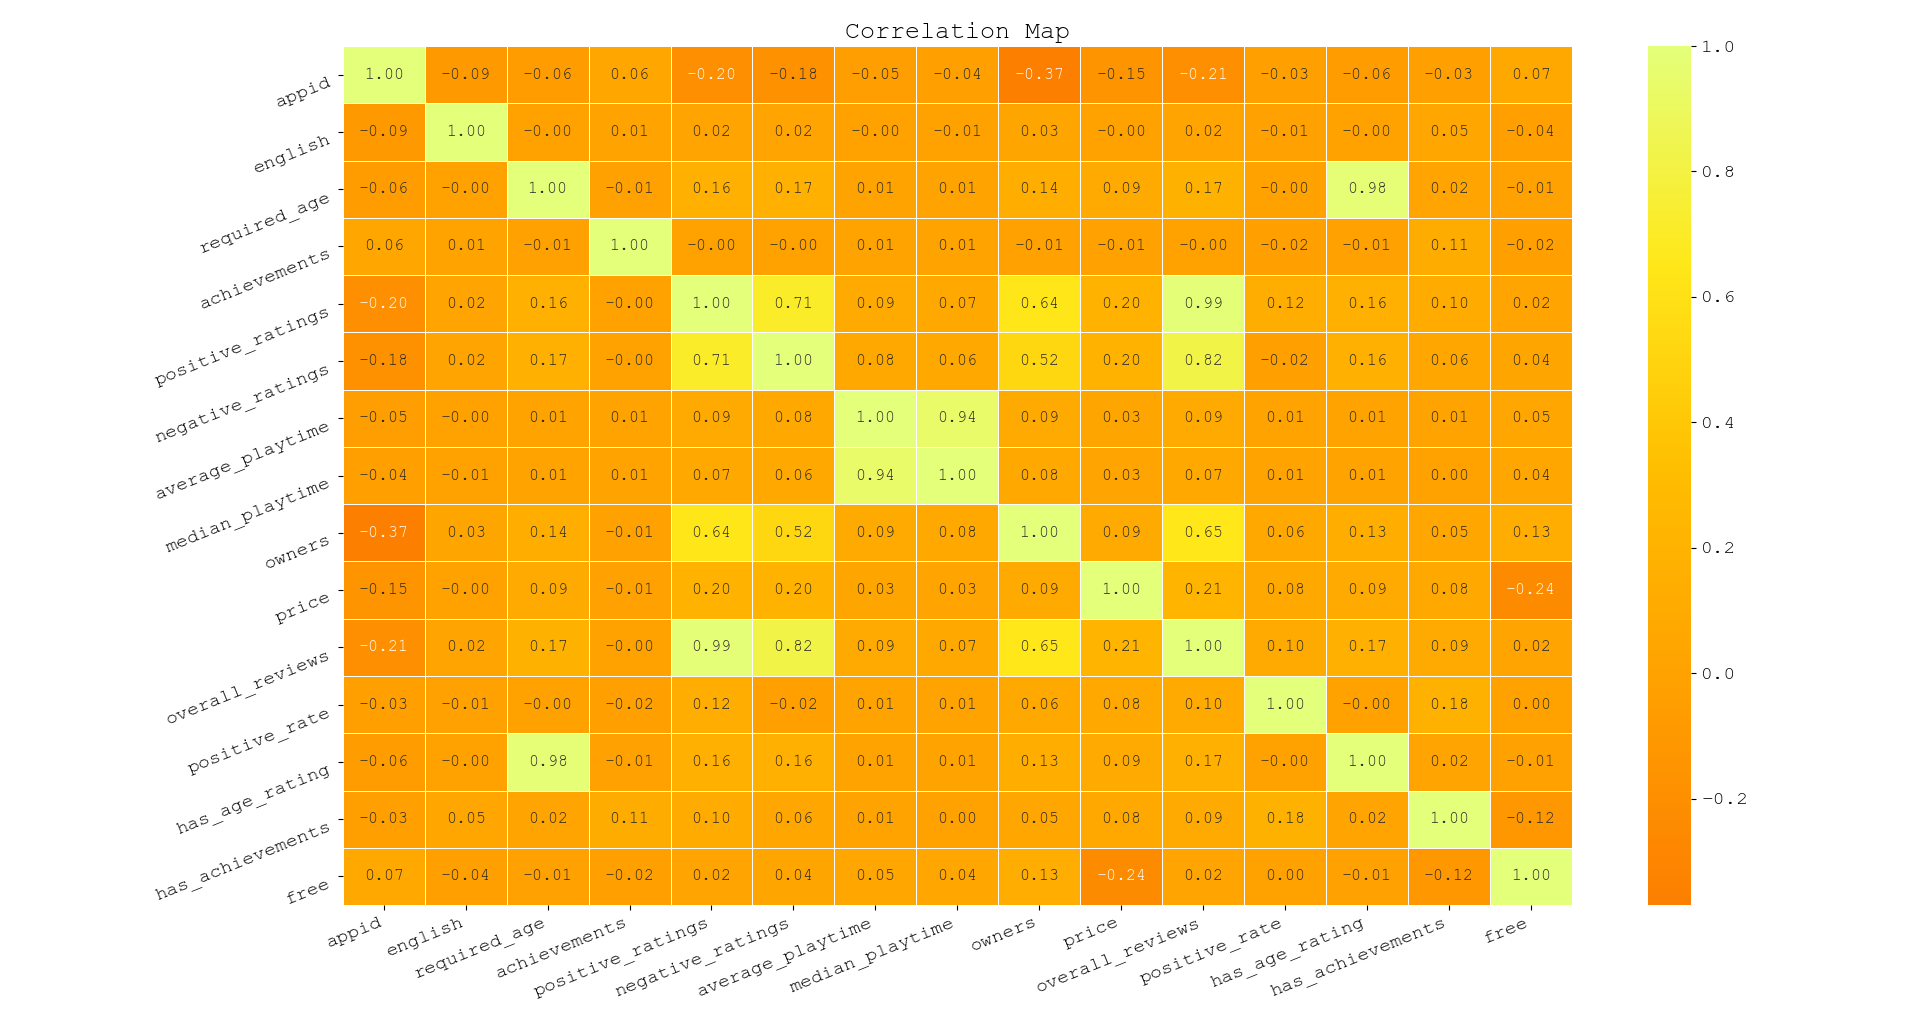
\includegraphics[width=\linewidth]{assets-2/correlation_map.png}
  \caption{Correlation Heatmap.}
  \label{fig:heatmap1}
\end{figure}
\FloatBarrier

\begin{figure}[h]
  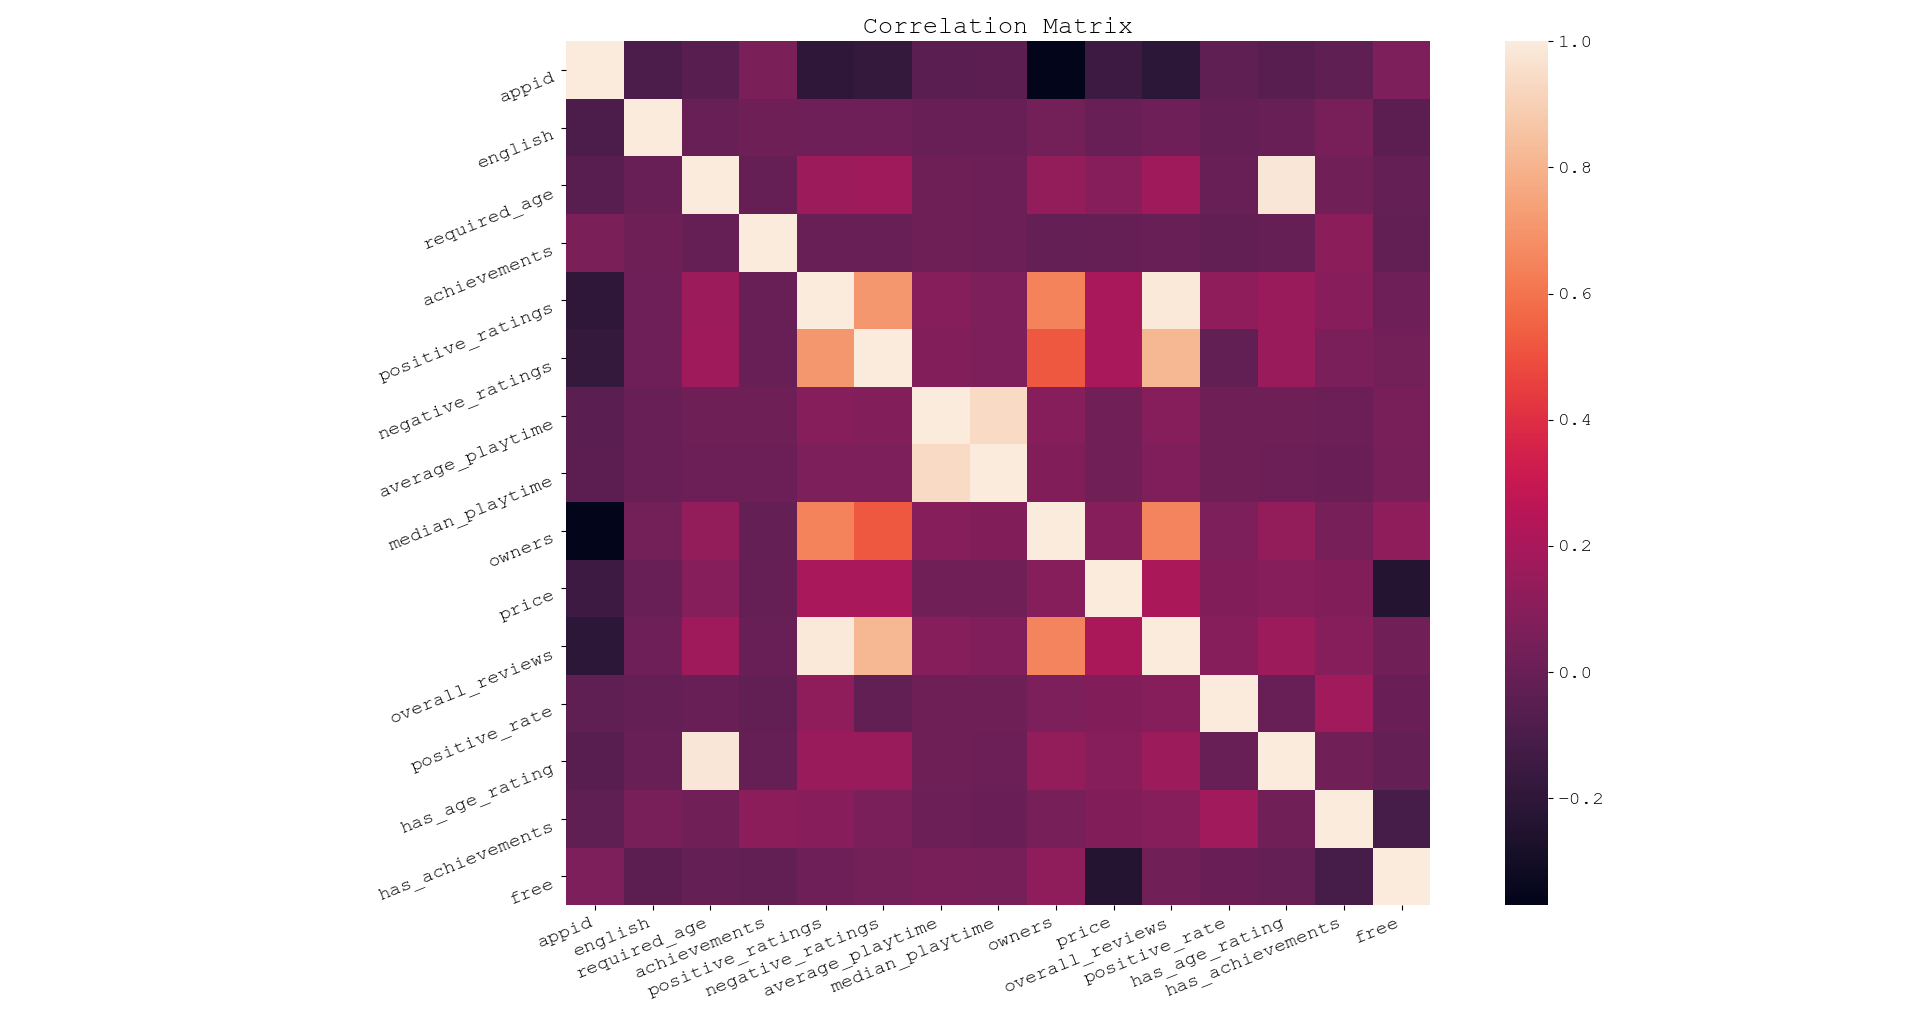
\includegraphics[width=\linewidth]{assets-2/correlation_matrix.png}
  \caption{Correlation Heatmatrix.}
  \label{fig:heatmap2}
\end{figure}
\FloatBarrier

By looking at the heatmap, we can say that the variables that the owners count is more dependent on are overall\_reviews, positive and negative reviews. In addition, it can be noticed that the achivements and price factors are also slightly dependent on this issue. Let's look at the scatter and regression plots related to the variables in the table. Let's examine their respective graphs. After that, we will observe how much non-quantitative variables depend by looking at theirs Box and Whiskers methods.

\begin{figure}[h]
  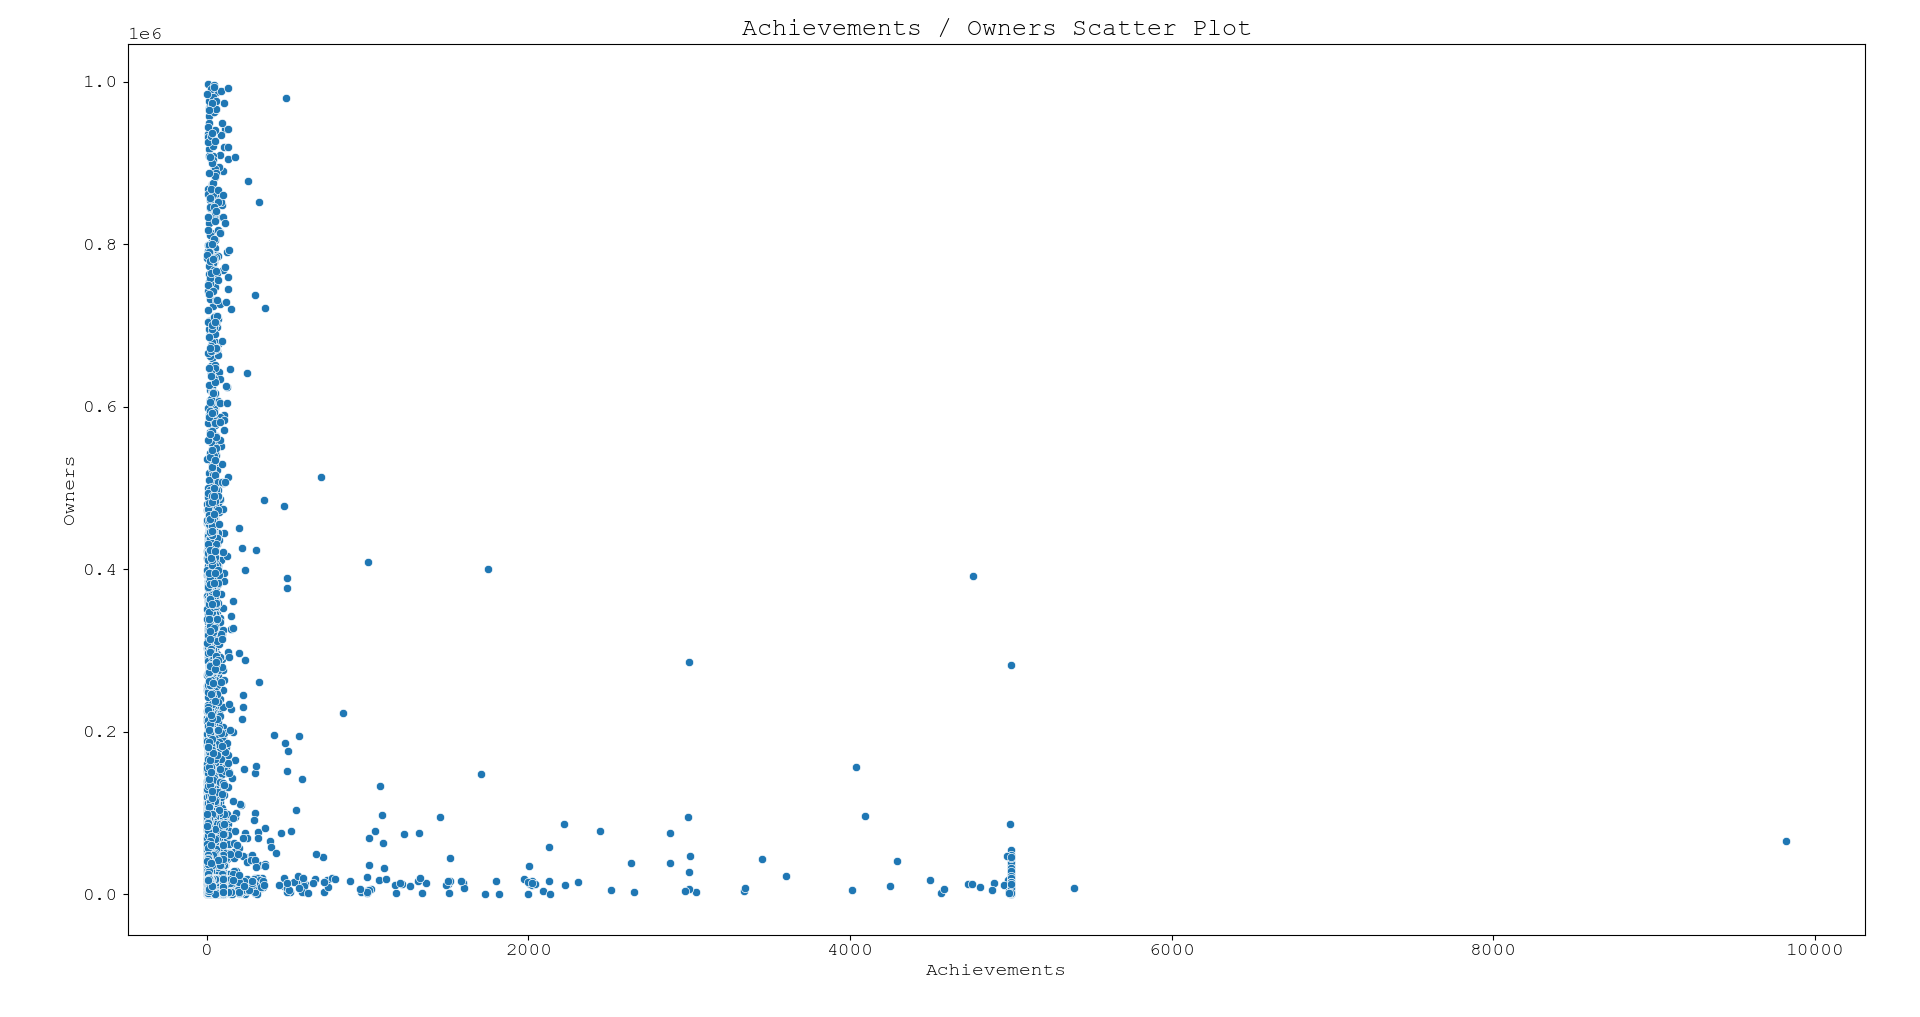
\includegraphics[width=\linewidth, height=3cm]{assets-2/achievements_owners_scatter.png}
  \caption{Scatter Plot of Achievements/Owners.}
  \label{fig:achievements_owners1}
\end{figure}
\FloatBarrier

\begin{figure}[h]
  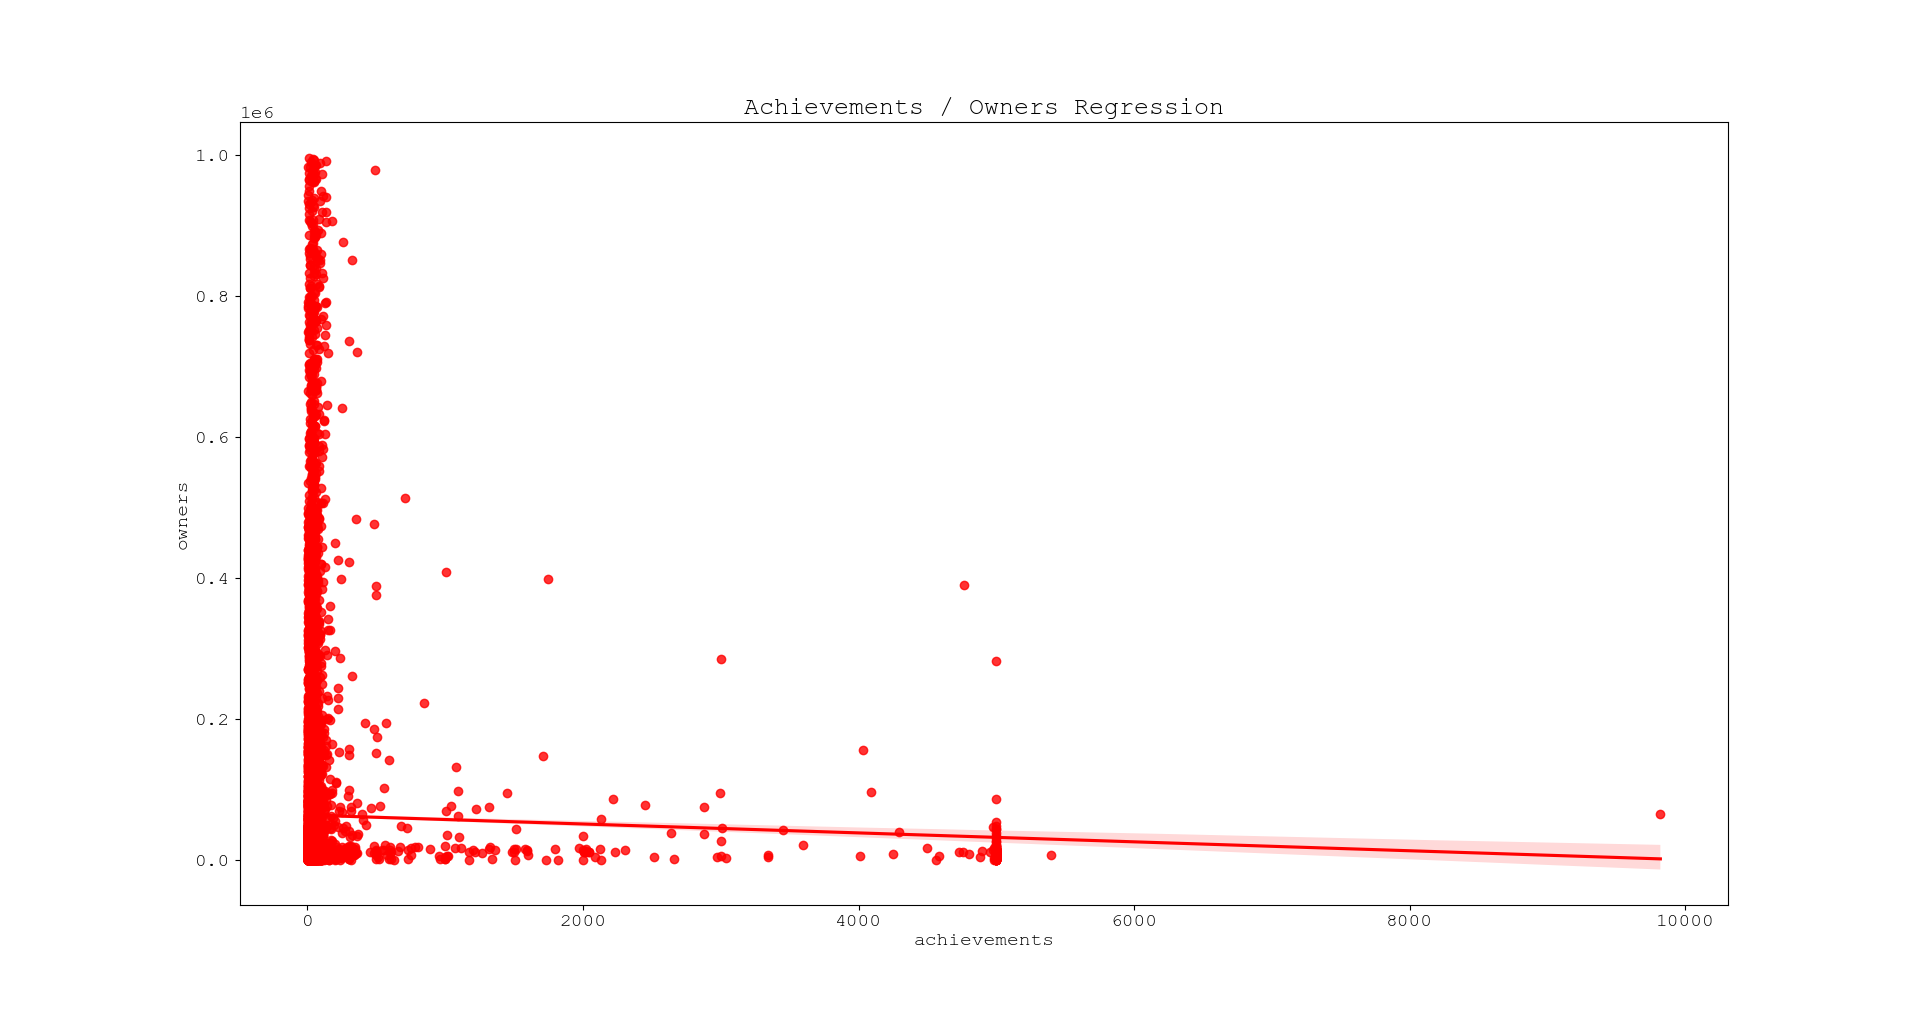
\includegraphics[width=\linewidth]{assets-2/achievements_owners_regression.png}
  \caption{Regression of Achievements/Owners.}
  \label{fig:achievements_owners2}
\end{figure}
\FloatBarrier

Based on the scatter and regression graphs, we can say that the achievements column has a negative effect on the number of owners. In addition, the has\_achievements column shows that the presence of achievements has a positive effect on the number of owners. Therefore, we can say that the presence of achievements in a game, but not using it more than necessary, is the situation that will affect the sales of the game in the most positive way.

\begin{figure}[h]
  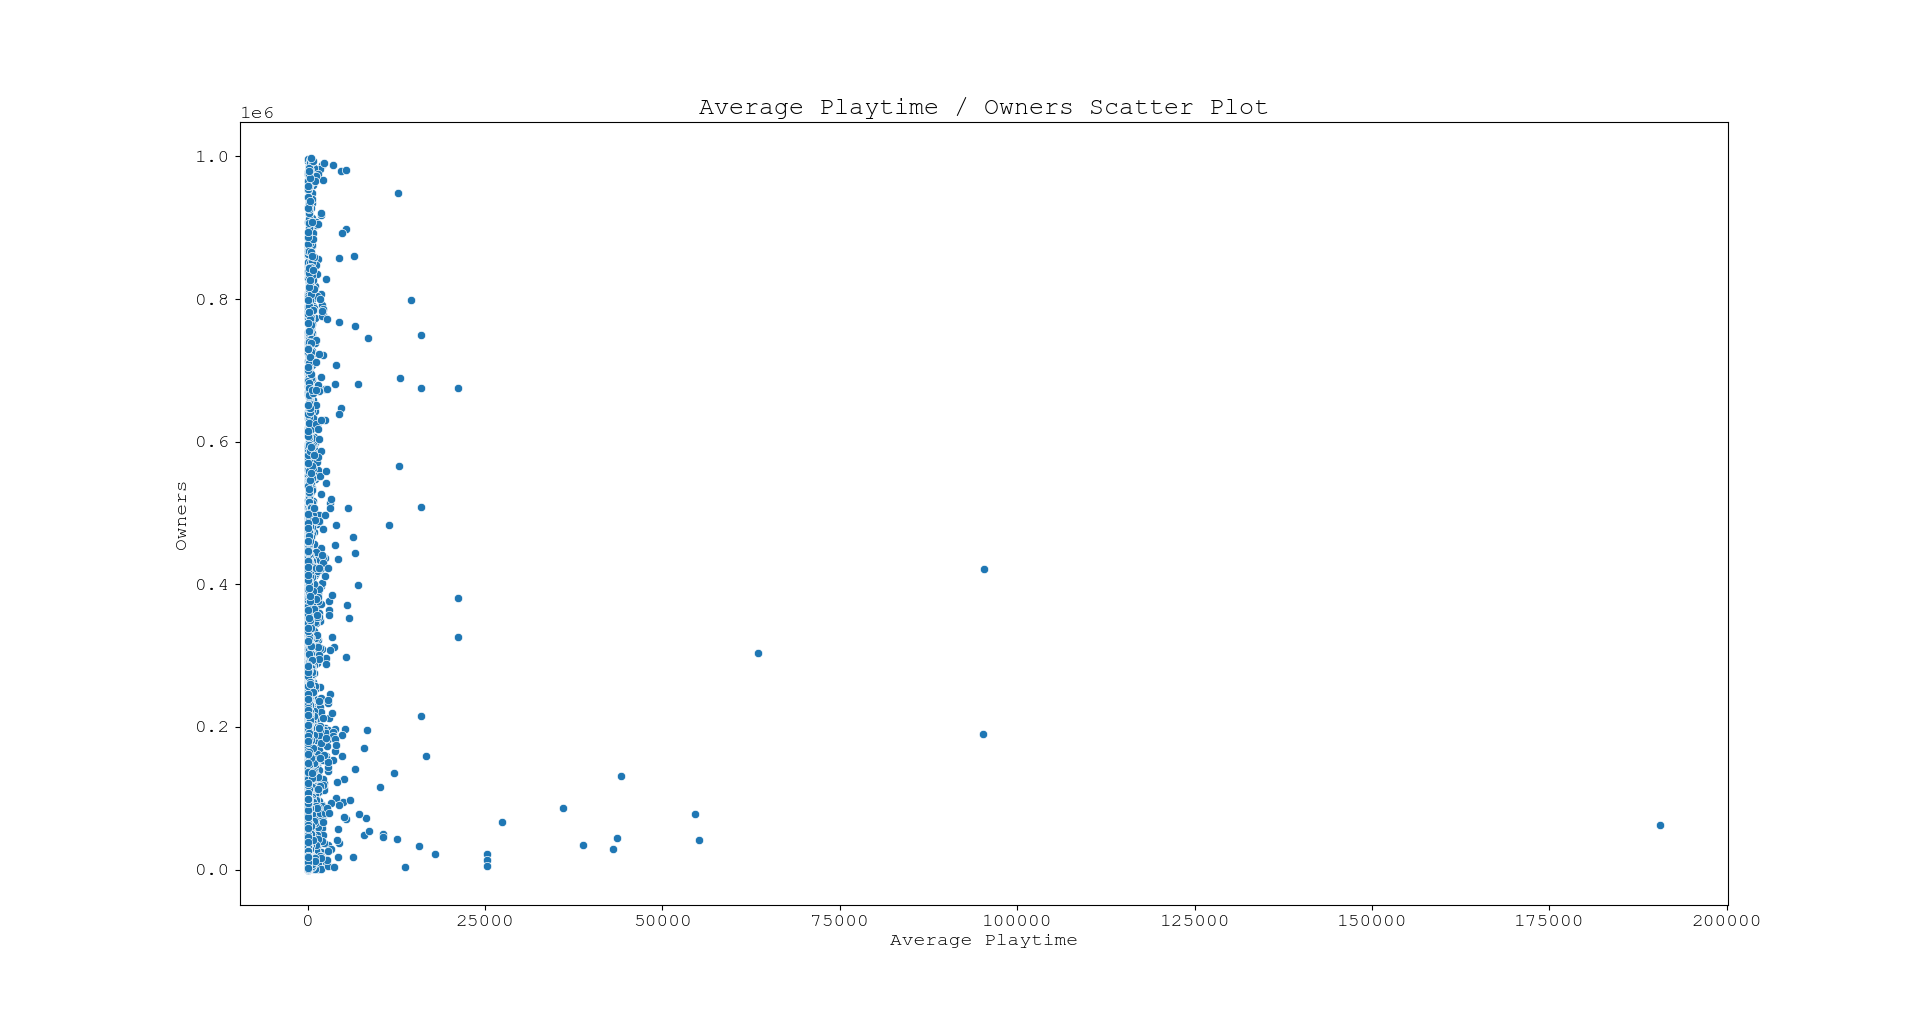
\includegraphics[width=\linewidth, height=6cm]{assets-2/average_playtime_owners_scatter.png}
  \caption{Scatter Plot of Average Playtime/Owners.}
  \label{fig:average_playtime_owners1}
\end{figure}
\FloatBarrier

\begin{figure}[h]
  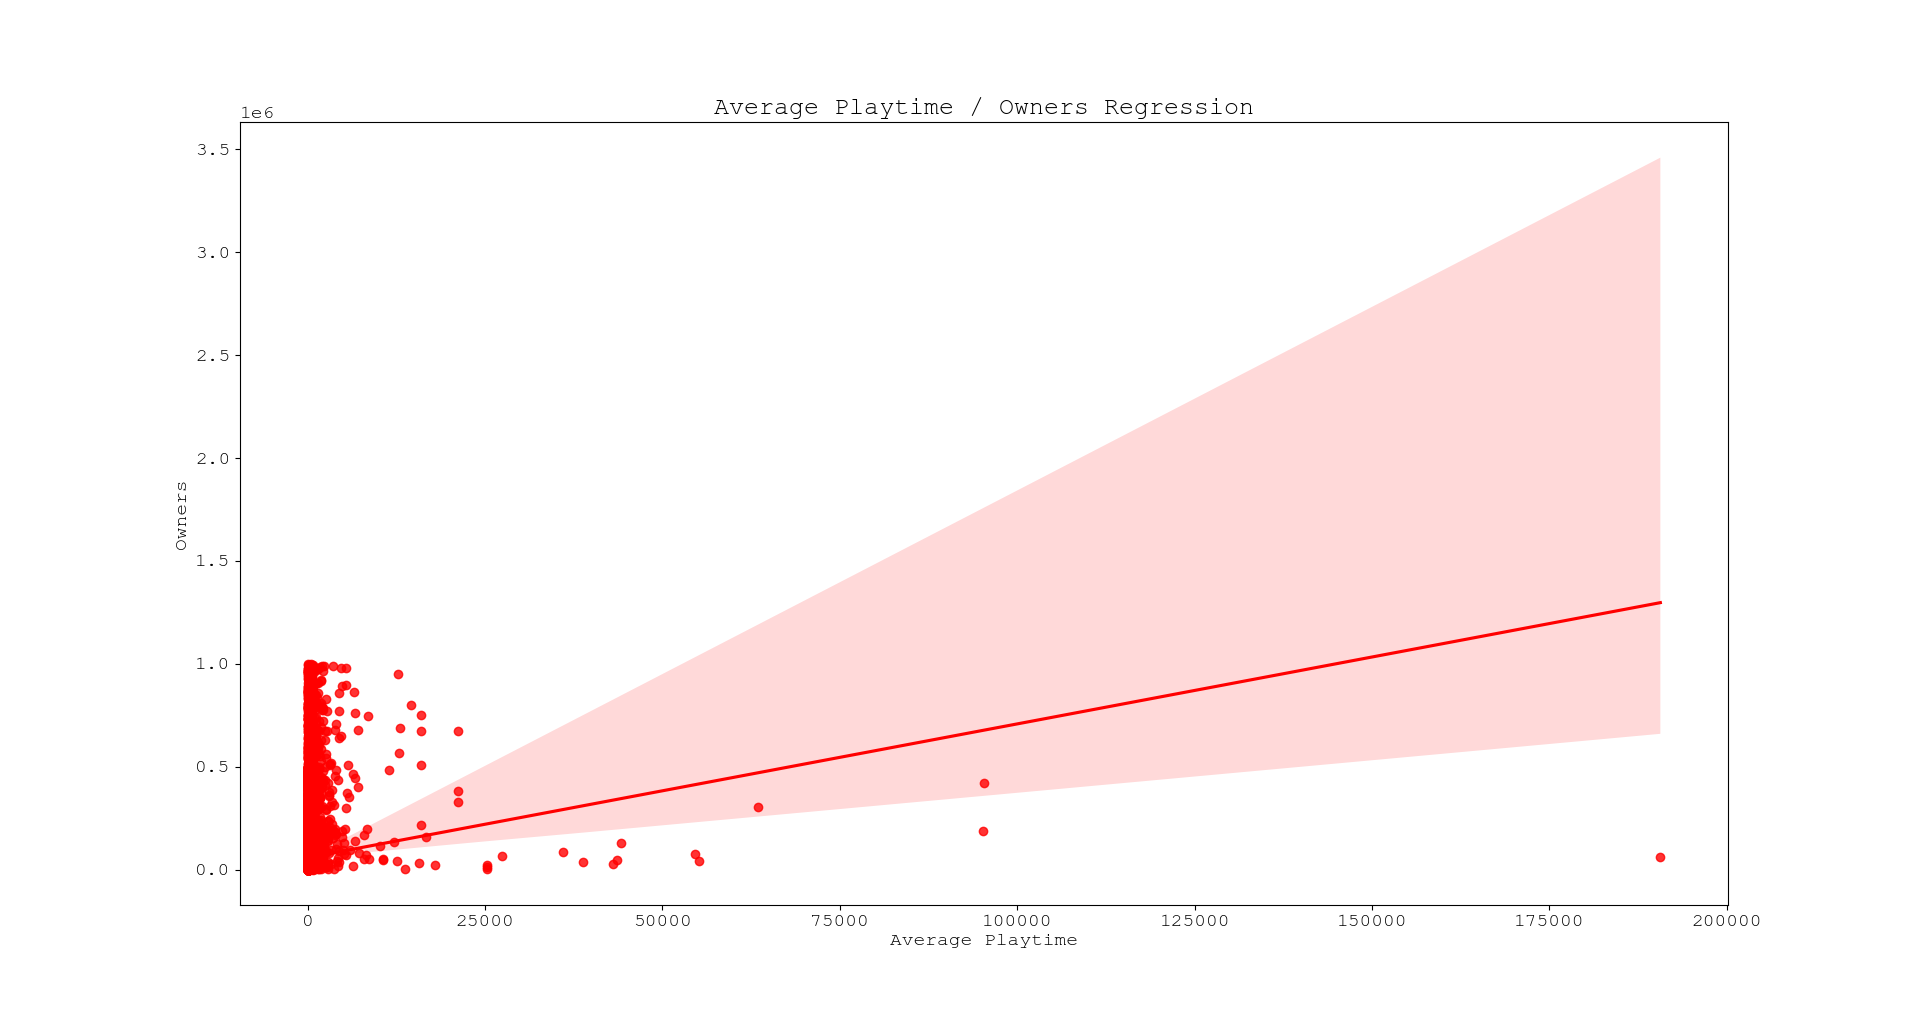
\includegraphics[width=\linewidth, height=5cm]{assets-2/average_playtime_owners_regression.png}
  \caption{Regression of Average Playtime/Owners.}
  \label{fig:average_playtime_owners2}
\end{figure}
\FloatBarrier

Based on the scatter and regression graphs, we can say that the average\_playtime column has a positive effect on the number of owners. However, the distribution of the majority of the games is in the part where the average playtime is close to 0. Therefore, we can say that a high average playtime will not adversely affect game sales.

\begin{figure}[h]
  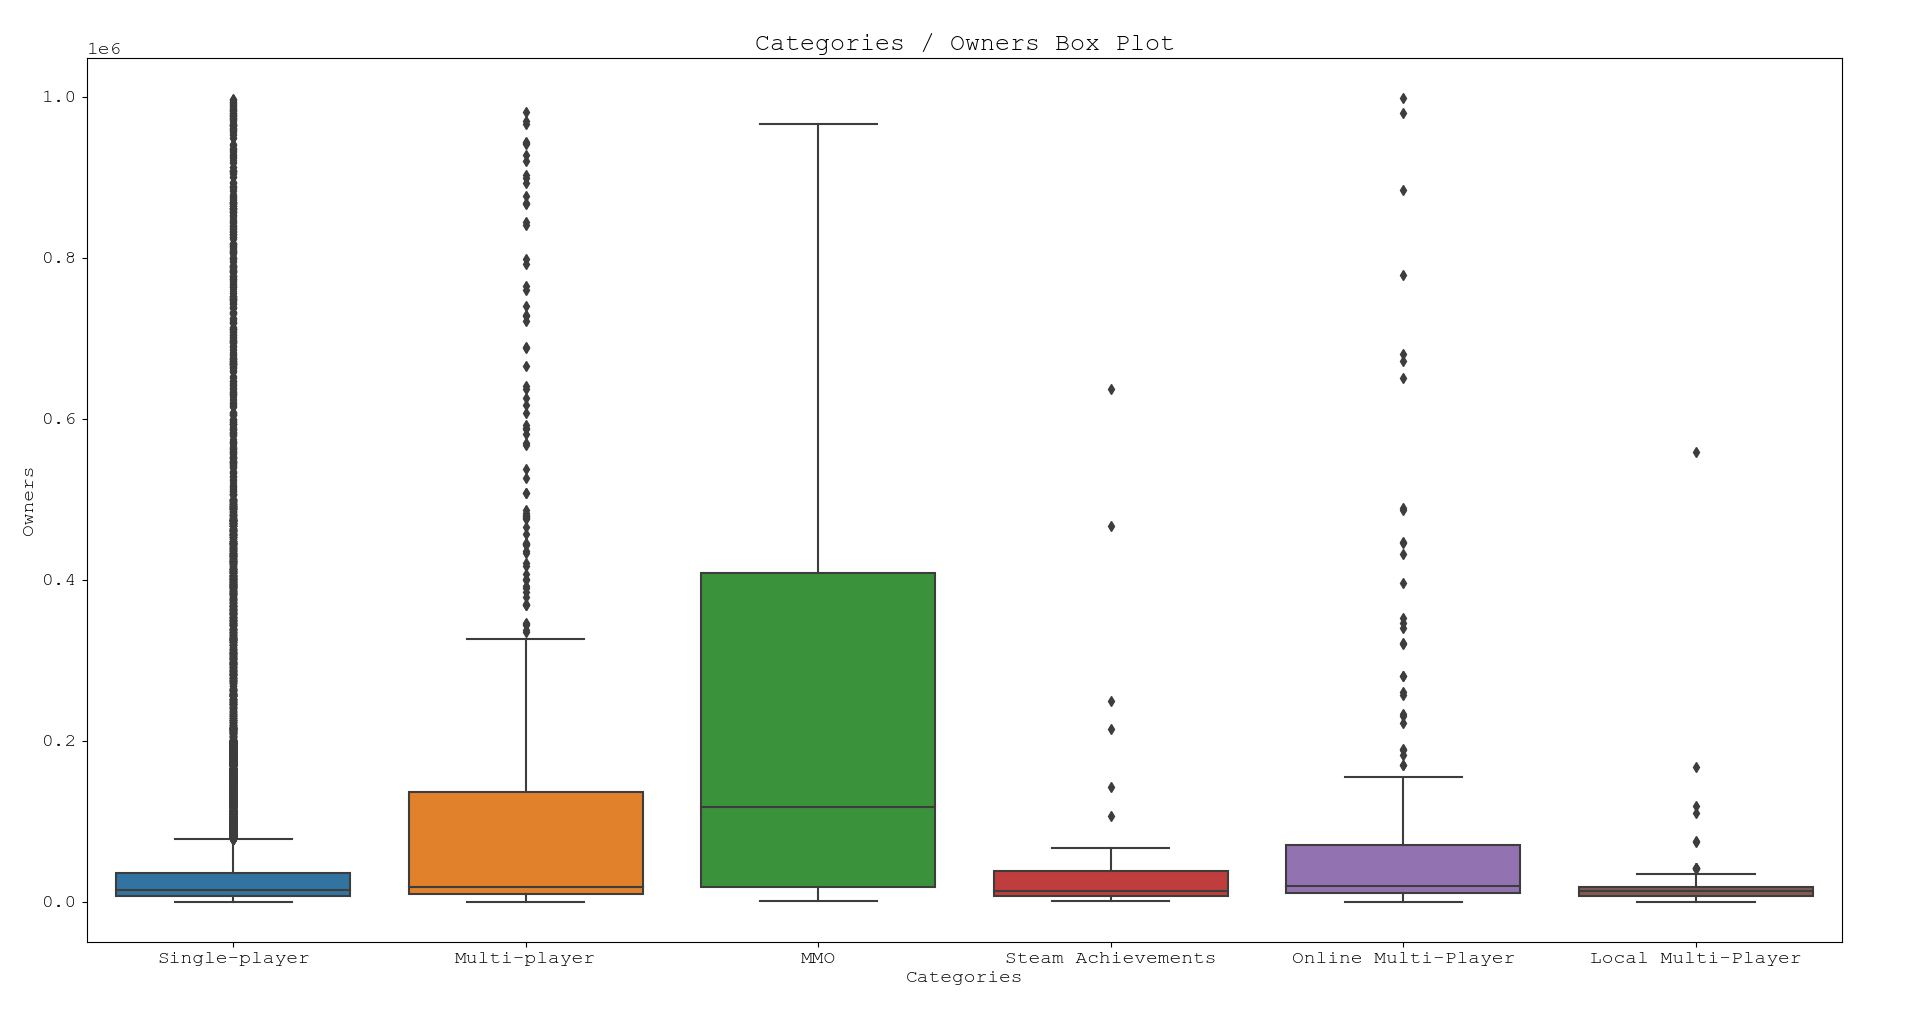
\includegraphics[width=\linewidth]{assets-2/categories_owners_box.png}
  \caption{Box Plot of Categories/Owners.}
  \label{fig:categories_owners1}
\end{figure}
\FloatBarrier

Based on the Categories/Owners box plot made for the 6 most existing categories, we can say that the MMO category has a wider spread and its median is superior to the other categories. We can say that the reason for this is that the games in the MMO category are usually free games. The Single Player category, which is the most common category in our dataset, tells us something different. It is impossible to say how this category can directly affect the sales of a game due to the presence of so many. Although we say that the median value is in under-owned games, we have a lot of outliers. The Multi Player category, which is the third category to be examined, is somewhere between Single Player and MMO. Although its median and distribution is similar to the Single Player category with low sales, it is more similar to MMO with its maximum value and outliers.

\begin{figure}[h]
  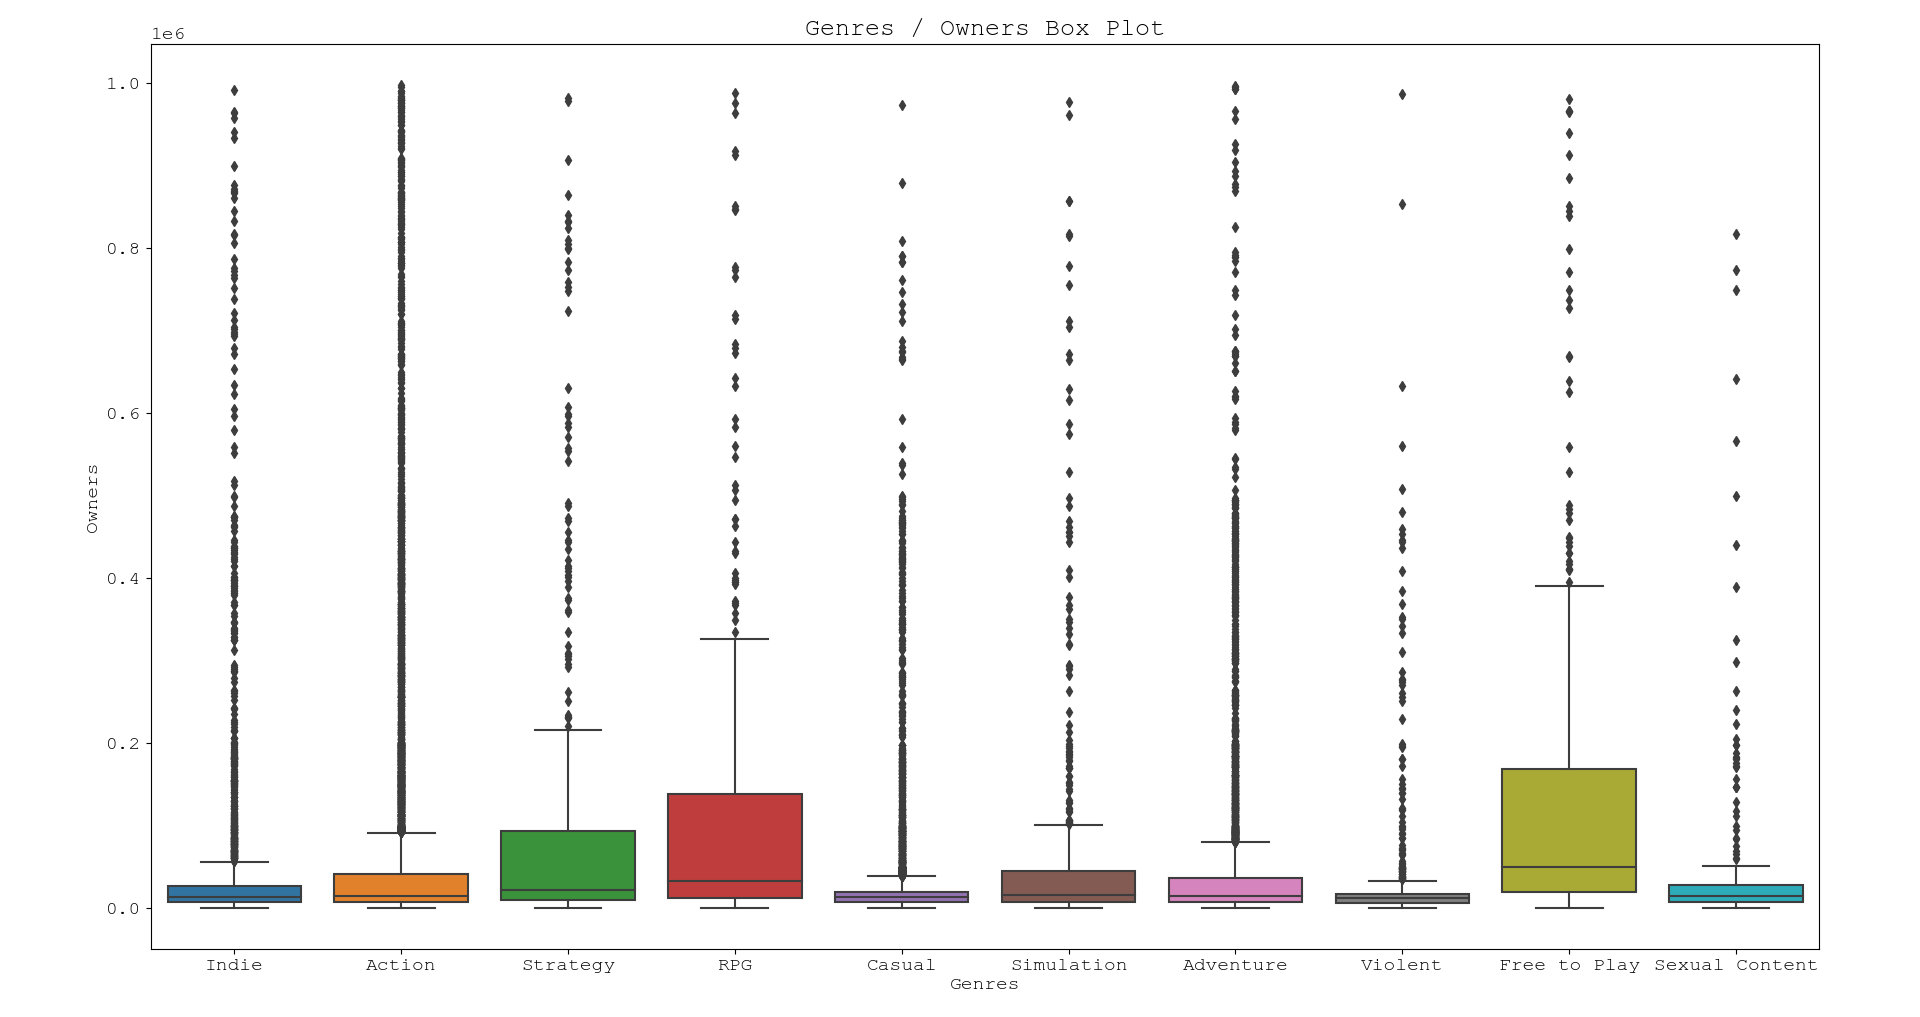
\includegraphics[width=\linewidth]{assets-2/genres_owners_box.png}
  \caption{Box Plot of Genres/Owners.}
  \label{fig:genres_owners1}
\end{figure}
\FloatBarrier

Based on the Genres/Owners box plot made on the top 10 existing genres, we can say that Free to Play and RPG genres (the fact that there is a similar data for that category, since there are genres in the MMO category, shows the accuracy of our graphics) have a wider spread and median is superior to other genres. We can say that this is due to the fact that these types of games are mostly free games. The most common genre in our dataset, the action genre, tells us something different. (Since the genre in the Single Player category is action in general, the fact that there is a similar data for that category shows the accuracy of our graphics.) It is impossible to say how this genre can directly affect the sales of a game due to the presence of too many. Although we say that the median value is in under-owned games, we have a lot of outliers. Strategy and Adventure genres, which can be examined as the 3rd, are somewhere between Action and Free To Play/RPG. Although its median and distribution are similar to the action genre in places with low sales, Free To Play/RPG is more similar with its maximum value and outliers.

\begin{figure}[h]
  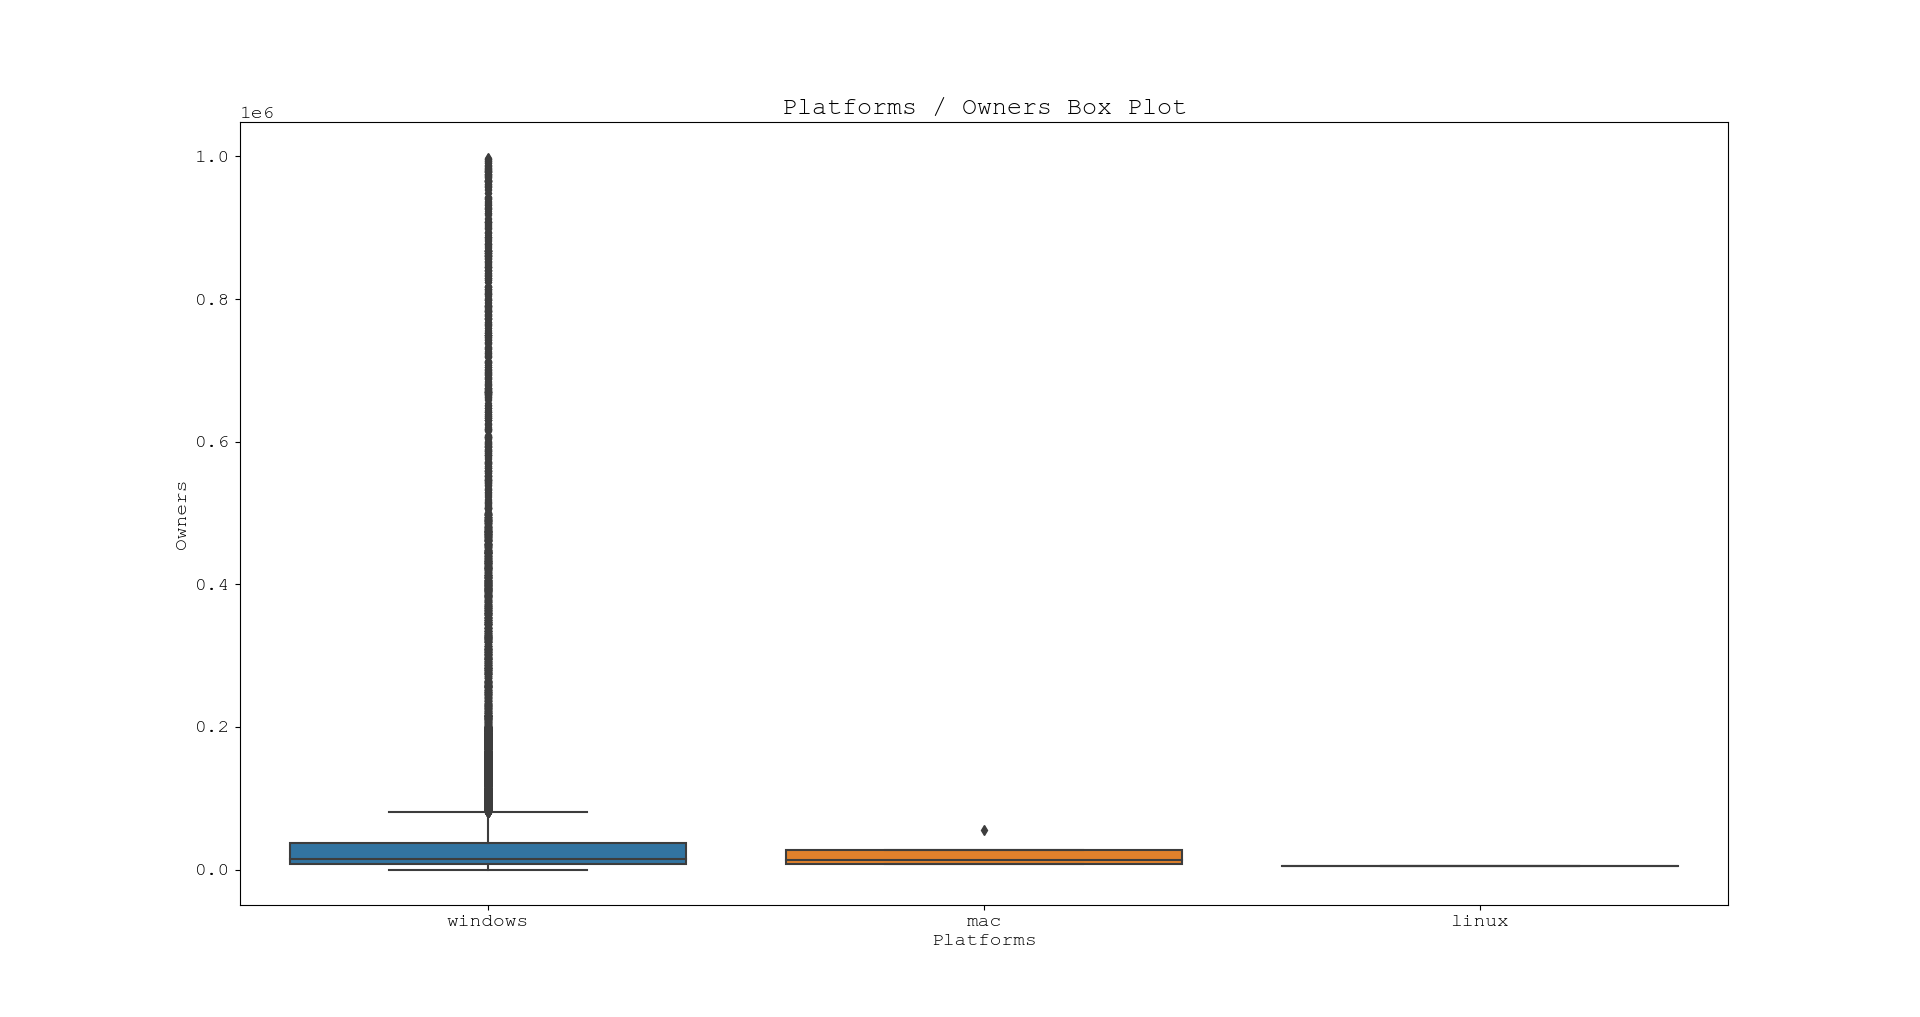
\includegraphics[width=\linewidth]{assets-2/platforms_owners_box.png}
  \caption{Box Plot of Platforms/Owners.}
  \label{fig:platforms_owners1}
\end{figure}
\FloatBarrier

Based on the Platforms/Owners box plot, we can say that the windows platform has a clear advantage over other platforms. However, this superiority does not have a positive effect on game sales. The fact that the game market is mostly carried out on this platform leaves us without comment on what effect it has on game sales.

\begin{figure}[h]
  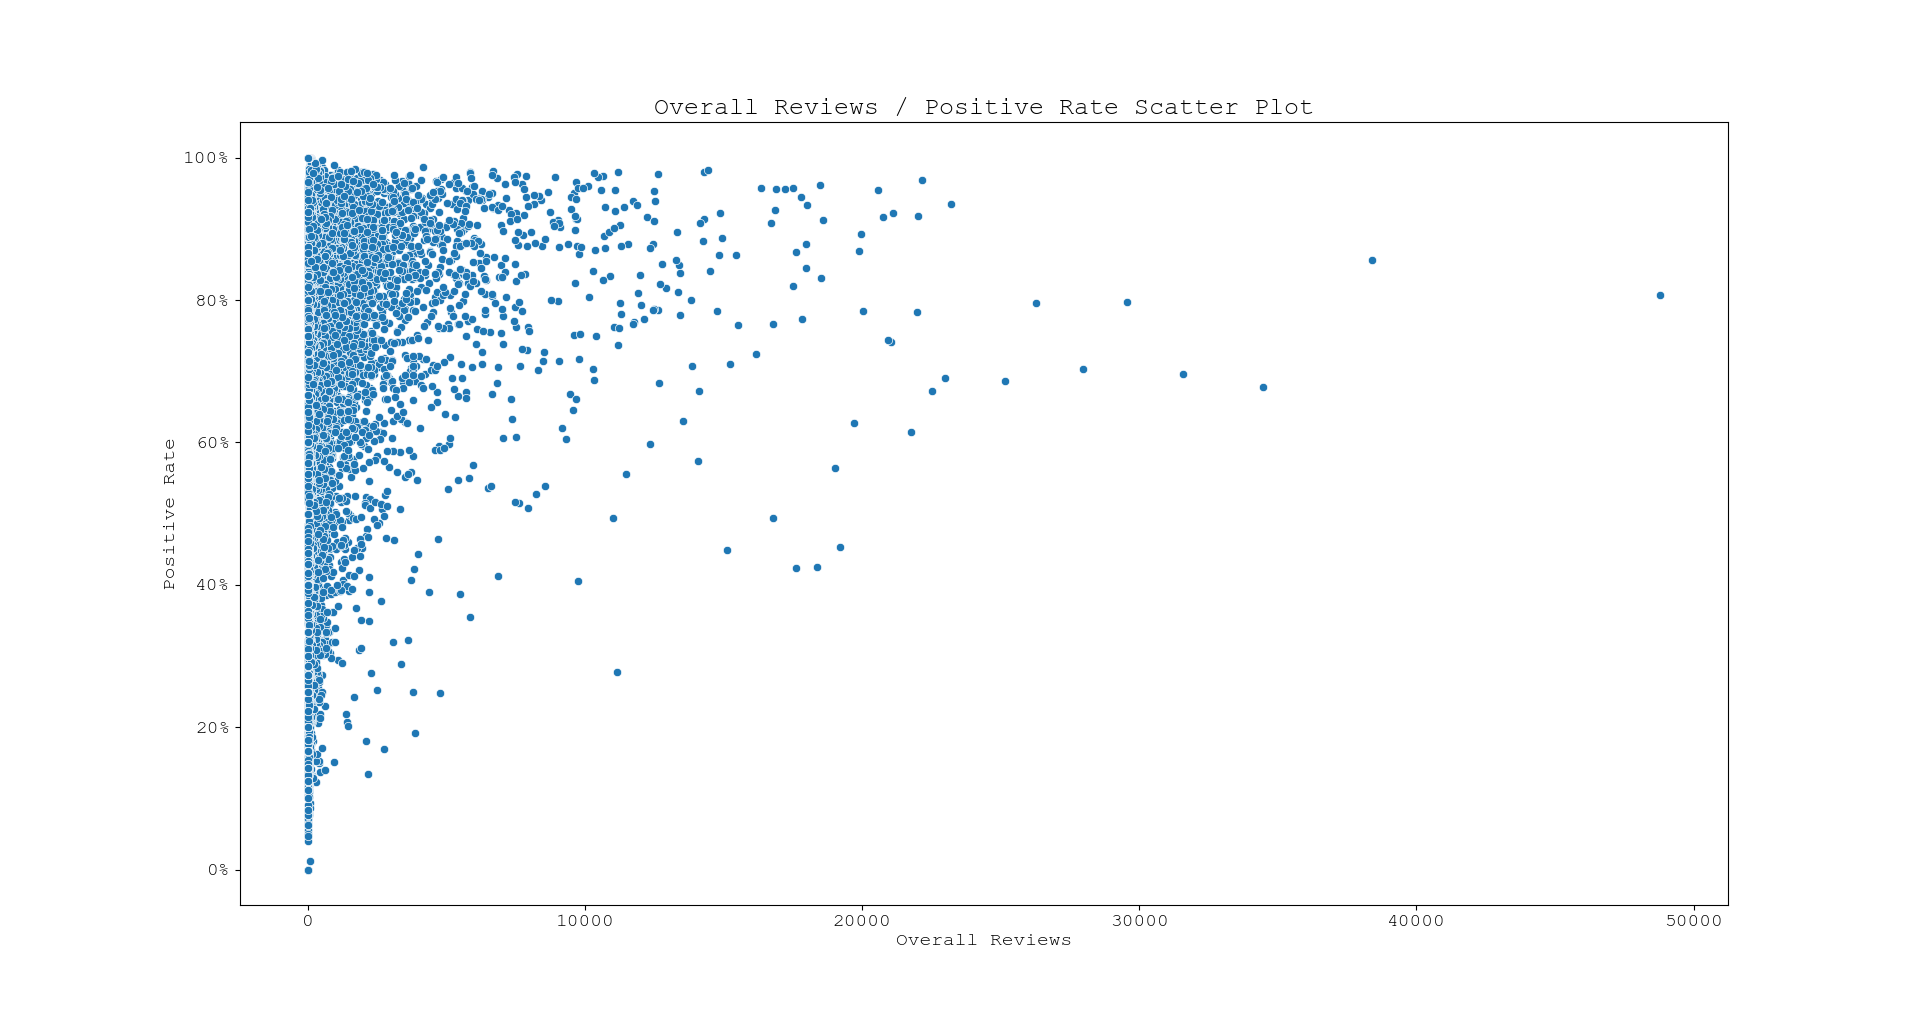
\includegraphics[width=\linewidth, height=5cm]{assets-2/overall_reviews_and_positive_rate.png}
  \caption{Scatter Plot of Overall Reviews/Positive Rate.}
  \label{fig:overall_reviews_positive_rate1}
\end{figure}
\FloatBarrier

Based on the Overall Reviews/Positive Rate scatter plot, the more users review a game, the more positive these reviews show. It is inevitable that more popular games sell more, so more people review the game. Now let's examine the effect of the positive rate column on game sales.

\begin{figure}[h]
  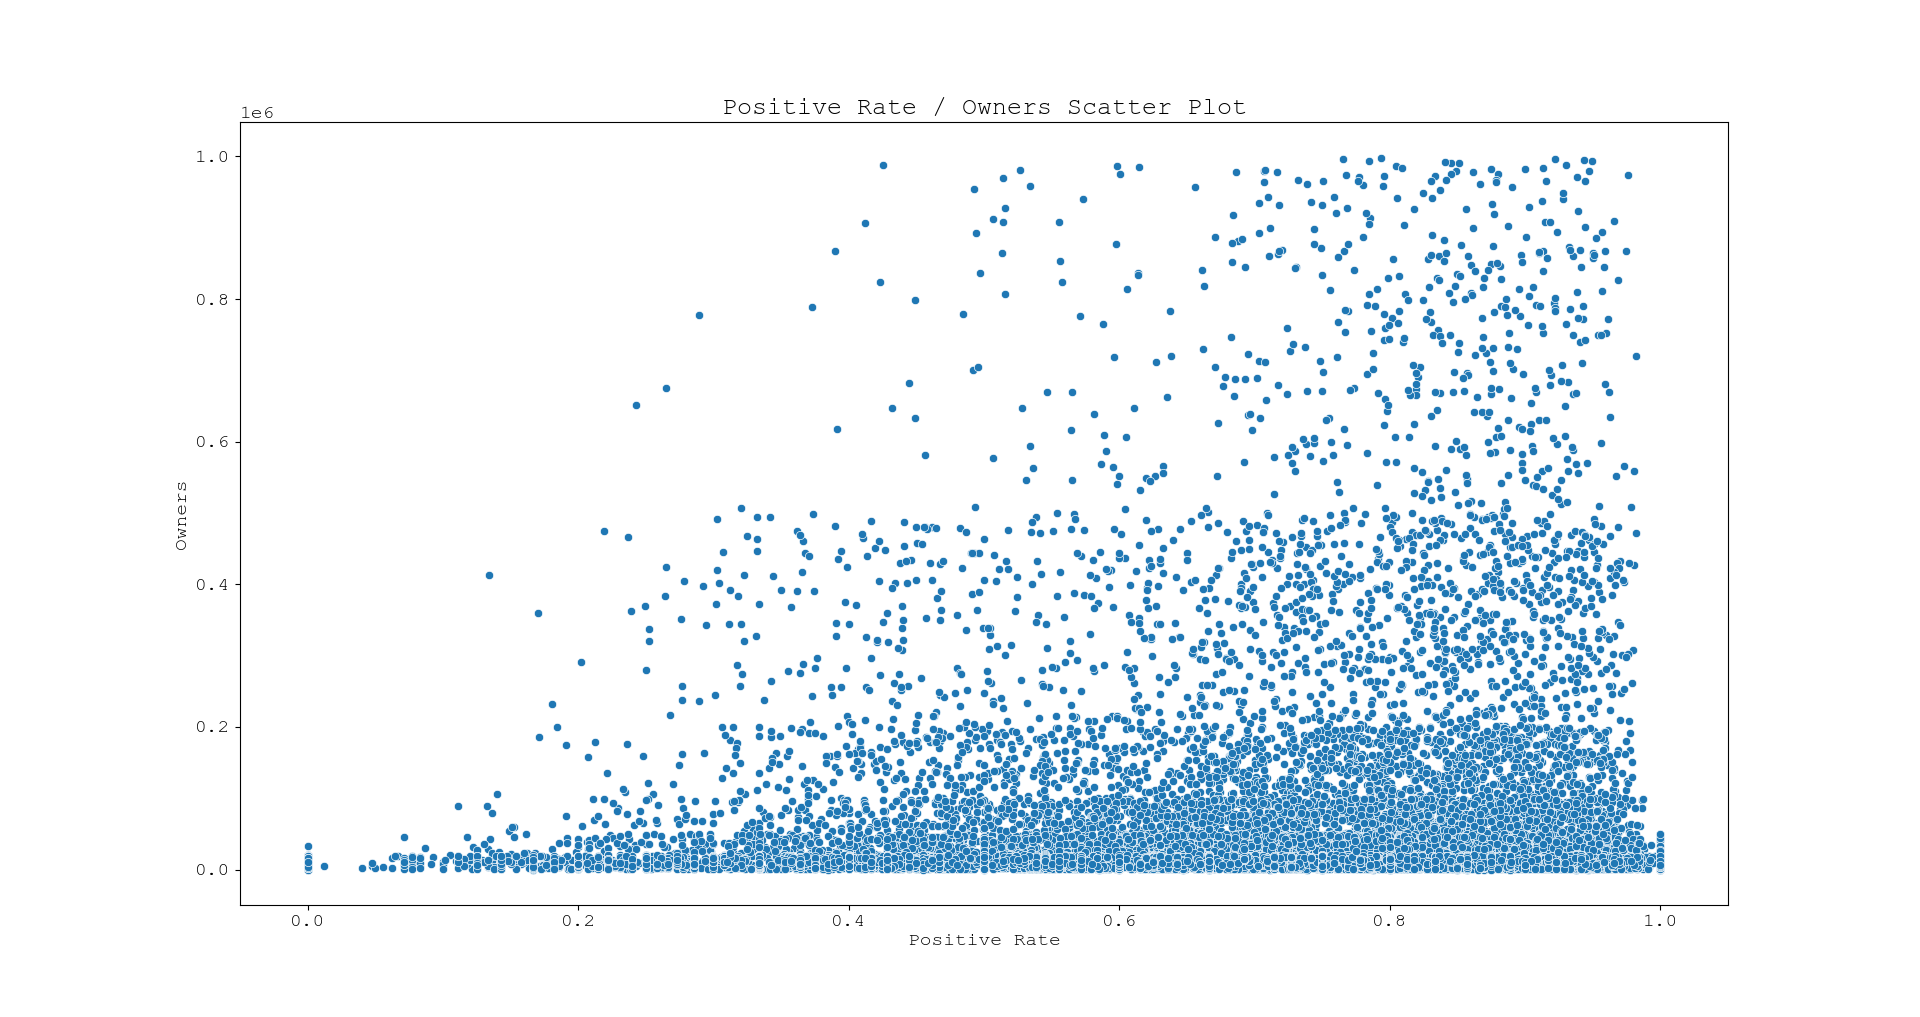
\includegraphics[width=\linewidth]{assets-2/positive_rate_owners_scatter.png}
  \caption{Scatter Plot of Positive Rate/Owners.}
  \label{fig:positive_rate_owners1}
\end{figure}
\FloatBarrier

\begin{figure}[h]
  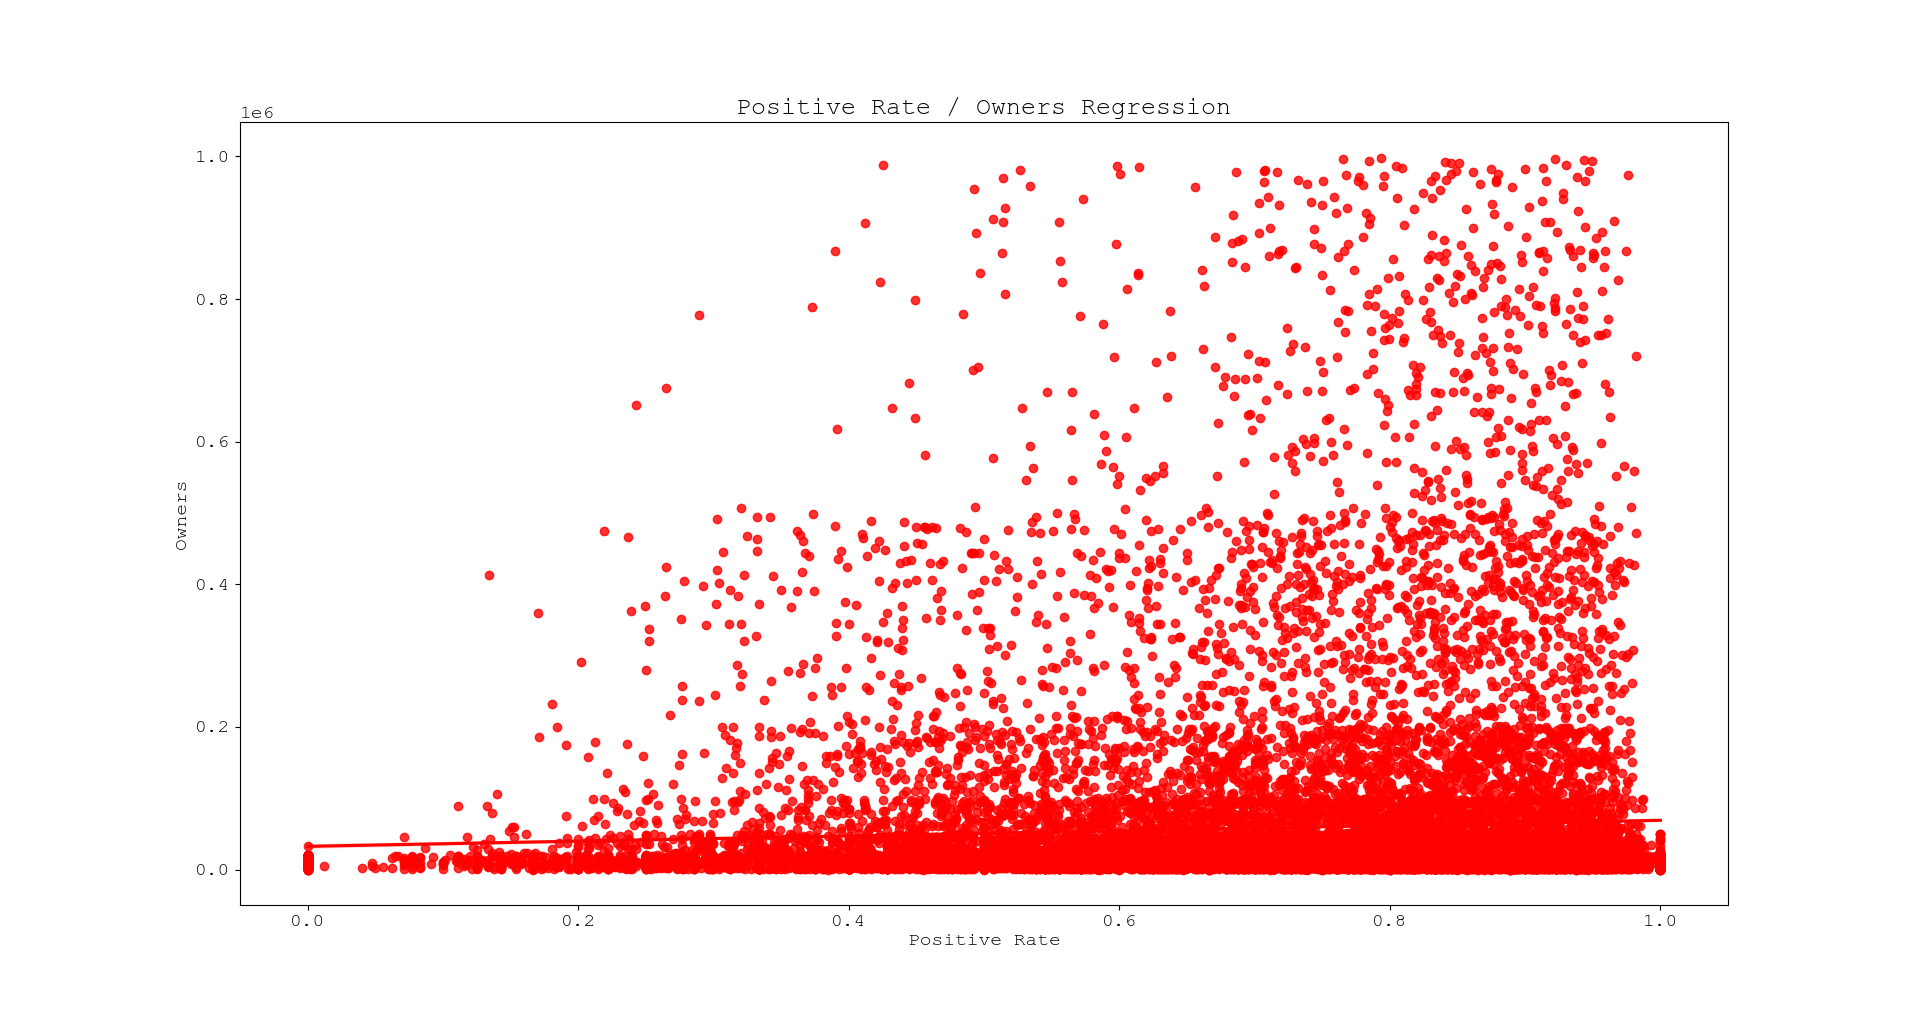
\includegraphics[width=\linewidth]{assets-2/positive_rate_owners_regression.png}
  \caption{Regression of Positive Rate/Owners.}
  \label{fig:positive_rate_owners2}
\end{figure}
\FloatBarrier

Based on the scatter and regression graphics, we can say that the positive\_rate column has a positive effect on game sales. The more positive reviews a game gets, the more likely it is to sell more games.

\begin{figure}[h]
  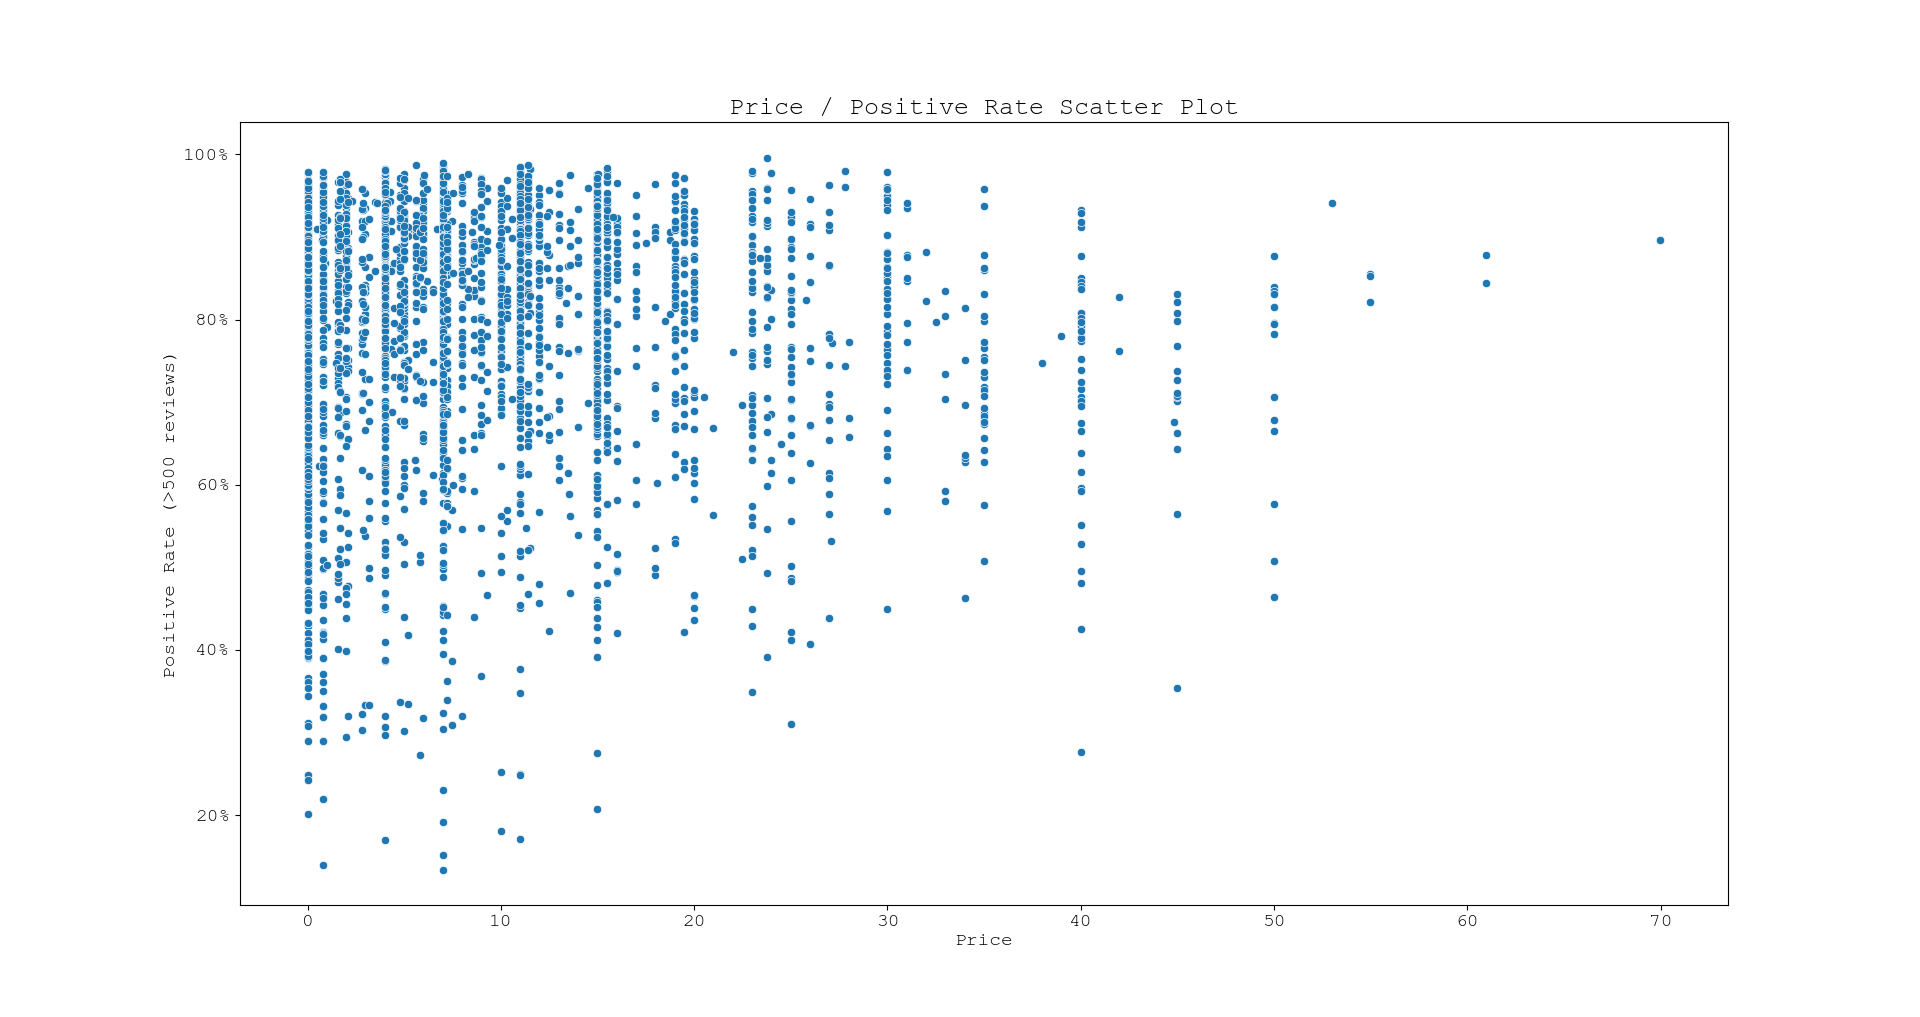
\includegraphics[width=\linewidth, height=6cm]{assets-2/price_and_positive_rate.png}
  \caption{Scatter Plot of Positive Rate/Price.}
  \label{fig:price_positive_rate1}
\end{figure}
\FloatBarrier

According to the Price/Positive Rate scatter plot, the more expensive a game is, the more positive reviews it gets. This is understandable, given that more expensive games are generally of higher quality. Now let's examine the effect of the price column on game sales.

\begin{figure}[h]
  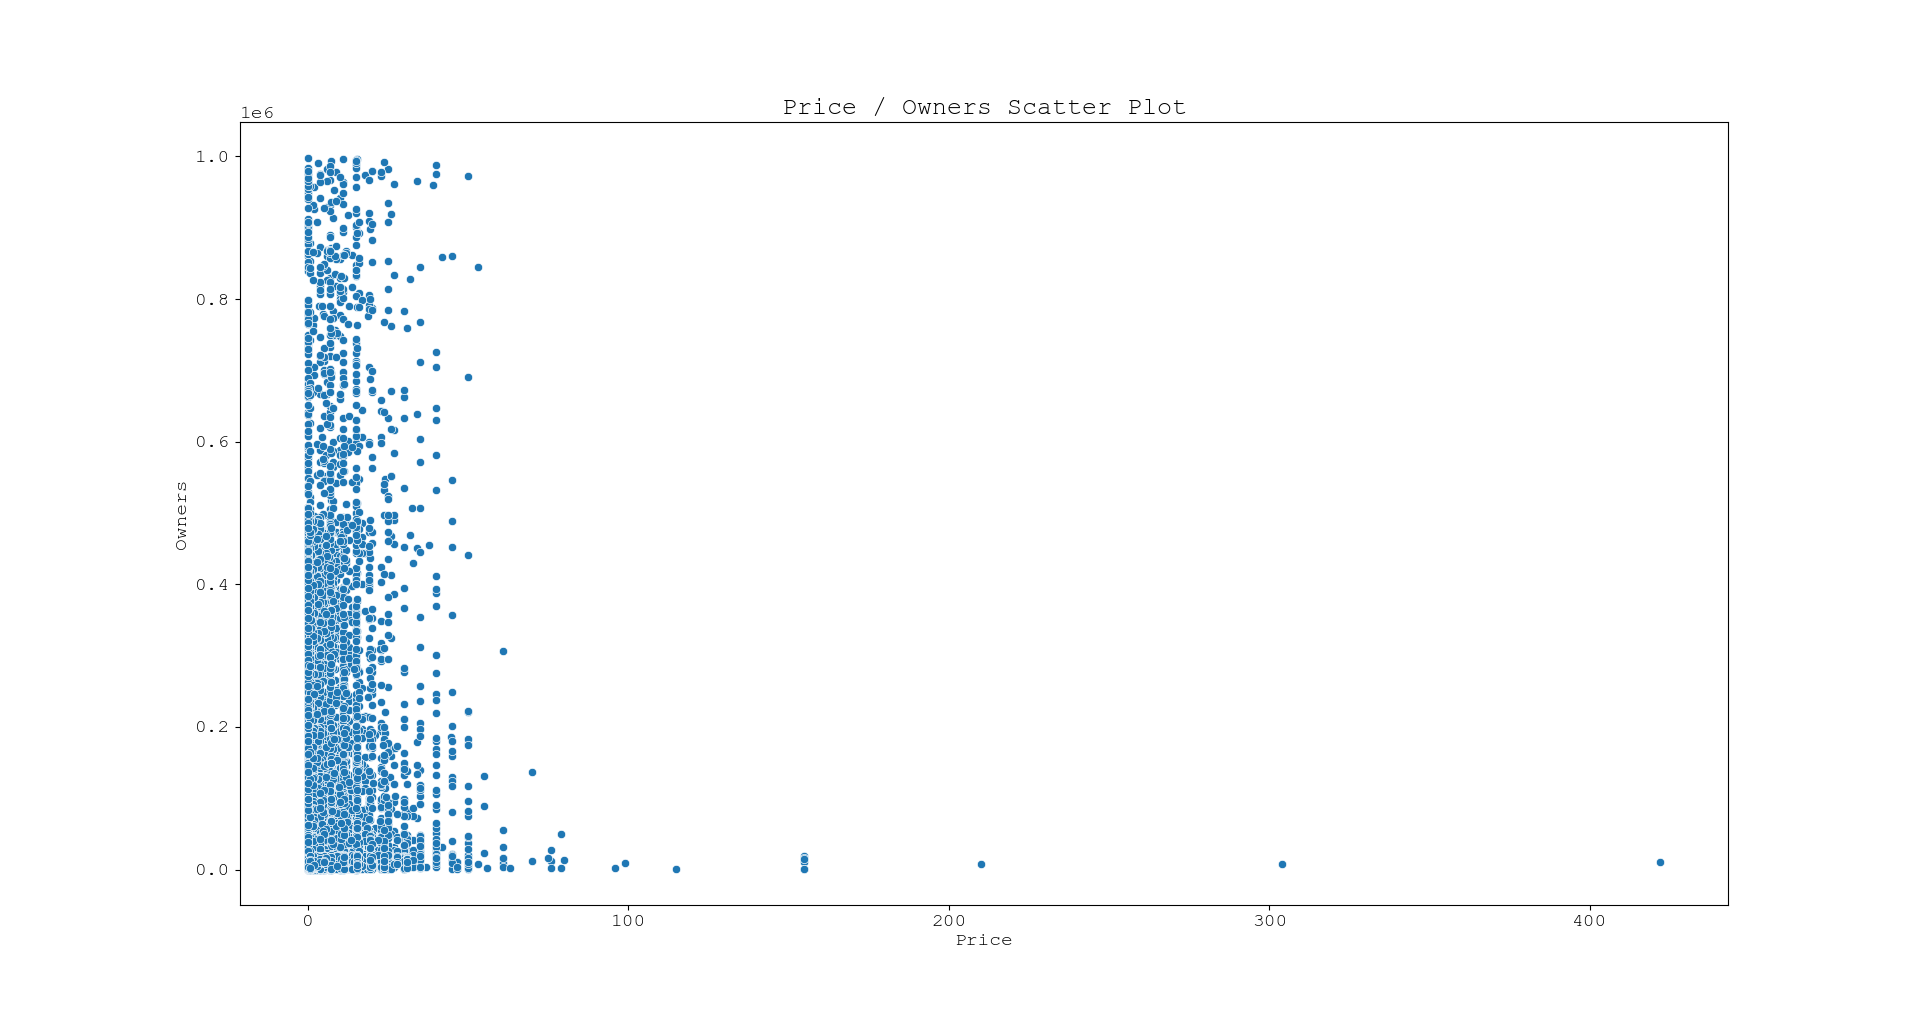
\includegraphics[width=\linewidth, height=9cm]{assets-2/price_owners_scatter.png}
  \caption{Scatter Plot of Price/Owners.}
  \label{fig:price_owners1}
\end{figure}
\FloatBarrier

\begin{figure}[h]
  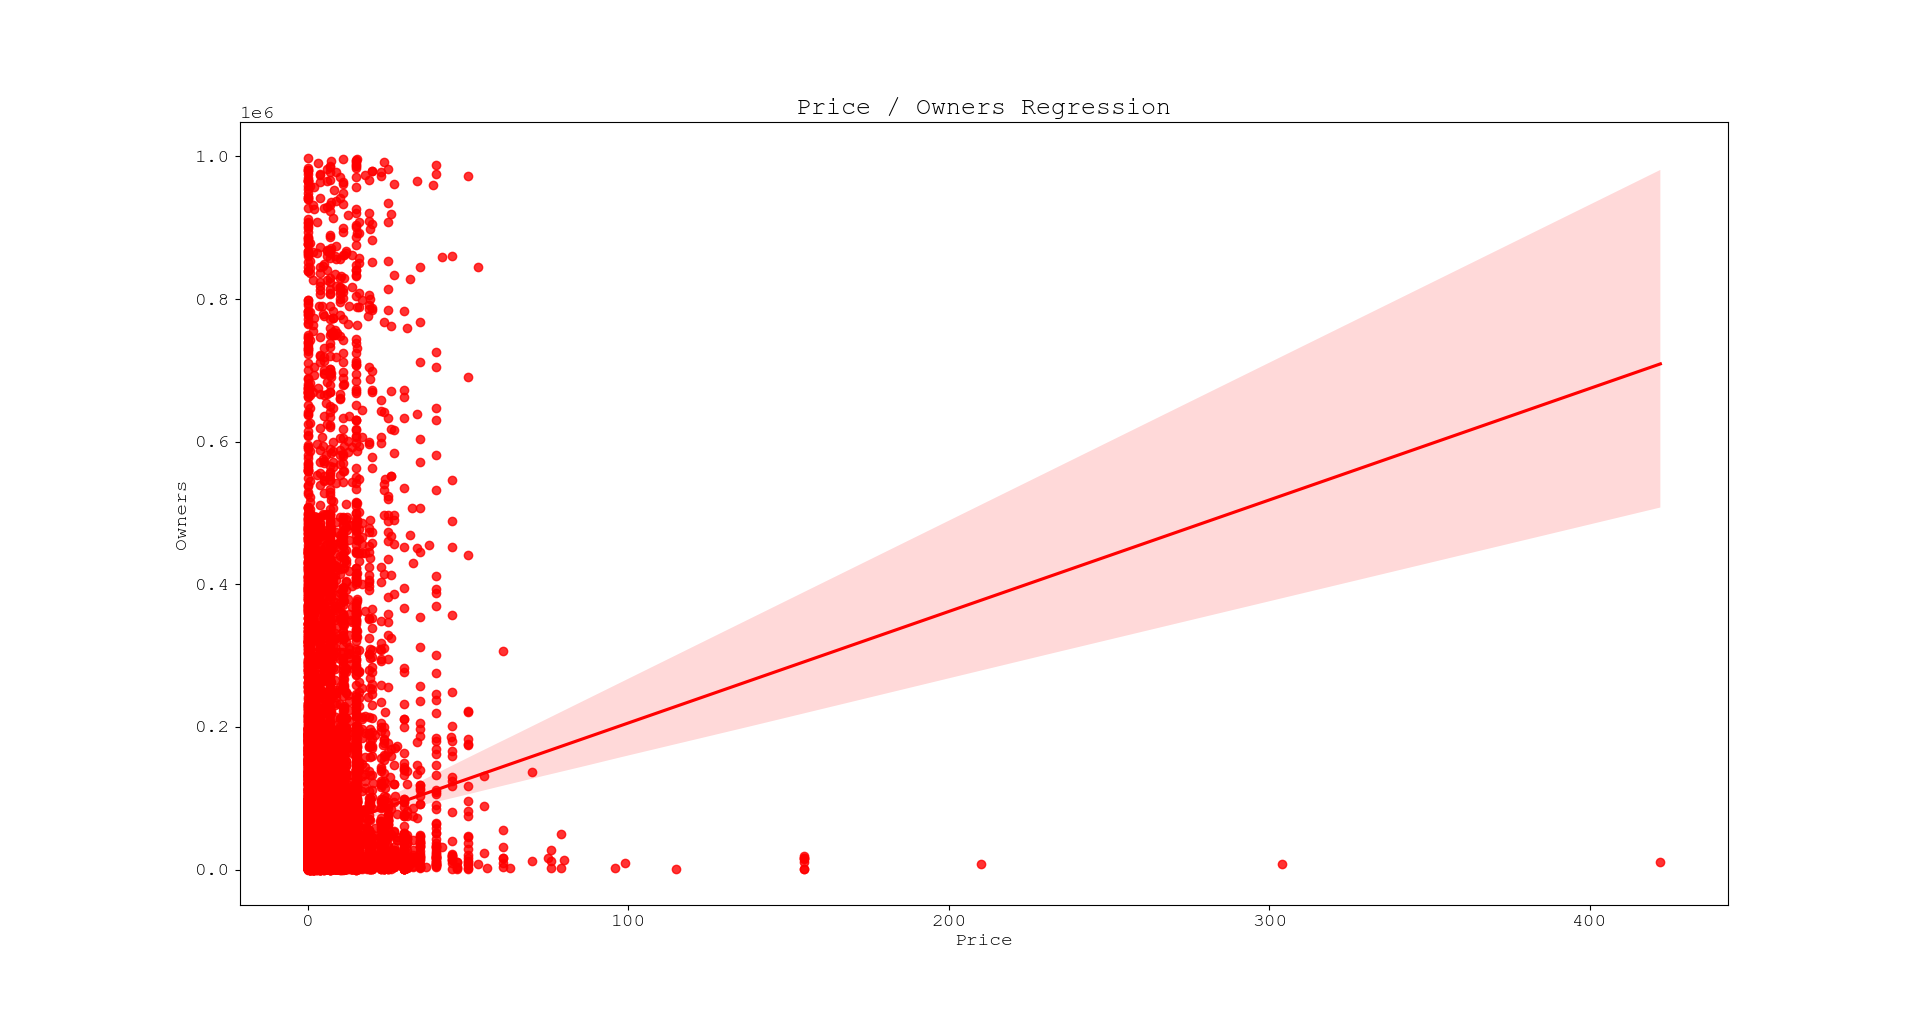
\includegraphics[width=\linewidth, height=9cm]{assets-2/price_owners_regression.png}
  \caption{Regression of Price/Owners.}
  \label{fig:price_owners2}
\end{figure}
\FloatBarrier

From the Price/Owners Count scatter and regression plots, we can say that the price column has a huge impact on game sales. And this effect is negative. The more expensive a game is, the fewer copies it sells. \\\\\\

\begin{figure}[h]
  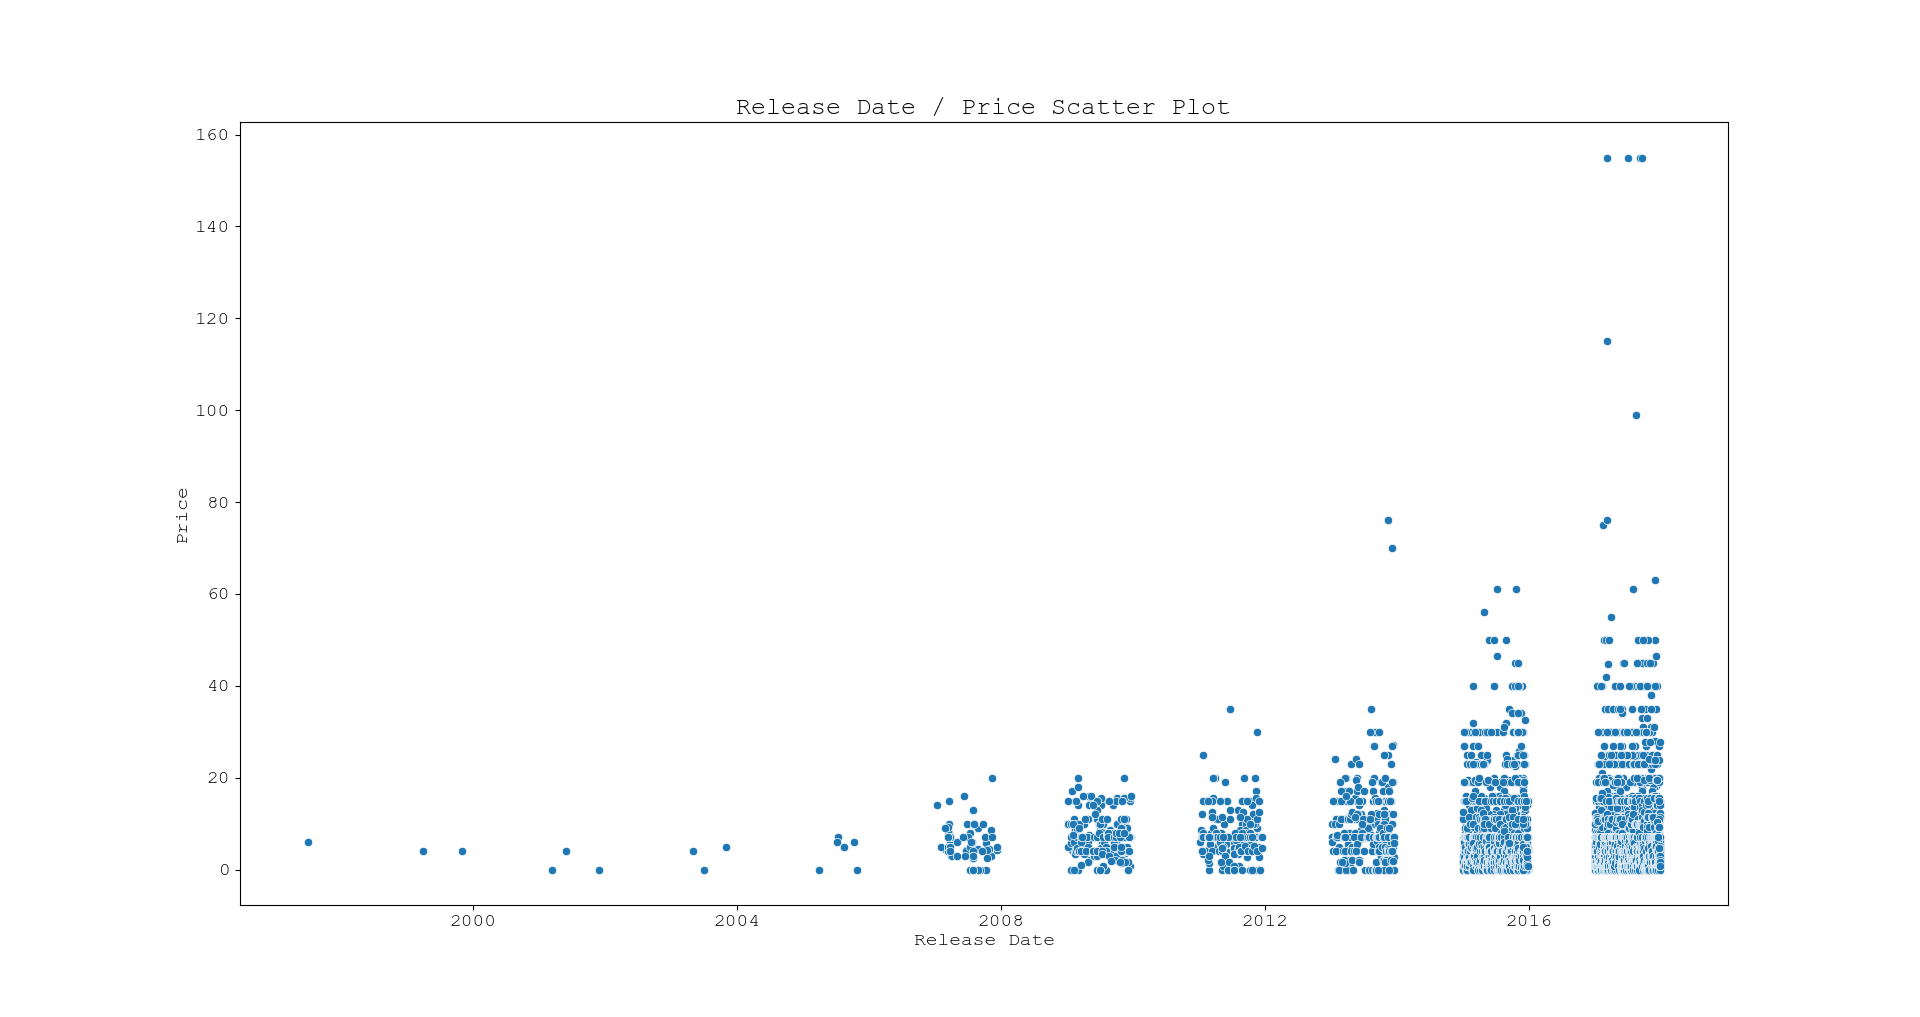
\includegraphics[width=\linewidth, height=5cm]{assets-2/release_date_price_scatter.png}
  \caption{Scatter Plot of Release Date/Price.}
  \label{fig:release_date_price1}
\end{figure}
\FloatBarrier

\begin{figure}[h]
  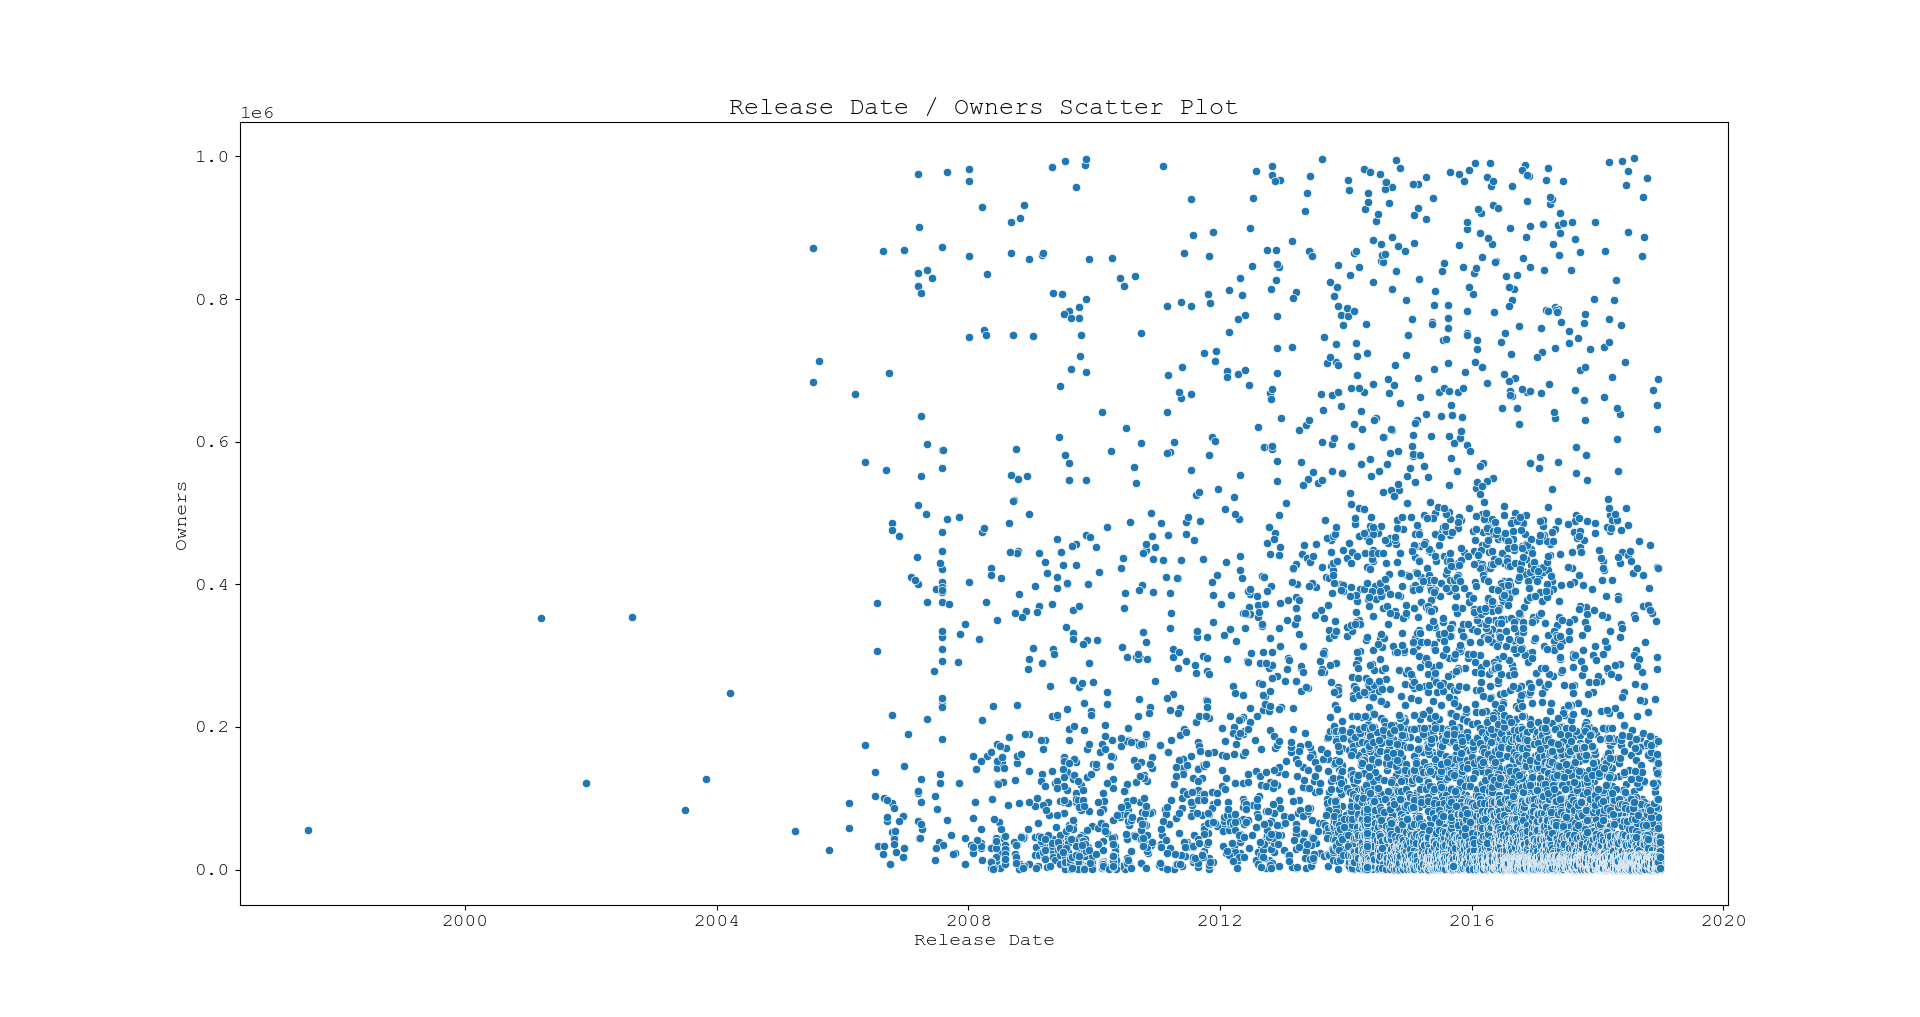
\includegraphics[width=\linewidth, height=5cm]{assets-2/release_date_owners_scatter.png}
  \caption{Scatter Plot of Release Date/Owners.}
  \label{fig:release_date_owners1}
\end{figure}
\FloatBarrier

By looking at the Price/Release Date and Release Date/Owners Count scatter plots, we can say that game prices are increasing as we approach 2020. We can say that the reason for this price increase is the increase in costs and inflation. Although the number of users increases as we approach 2020, we cannot observe that the games released in these years sell more games. We can say that the price column comes into play here.

\section{Conclusion}

Based on the univariate and multivariate features we examined, the scatter, box, bar, pie graphs we drew for them, and the correlation between them, we can reach the following conclusion.

An ideal video game should be released on the Windows Platform. The price must be low. Has Achievements but must have low achievement counts. There should be no age restriction. It should be in the Massively Multiplayer Online category, Free to Play and RPG genres (MMORPG for short). It should be a game with high overall reviews and English support.

In addition, these features have a vague effect on game sales: Platform, Single-player or Multiplayer categories, Action genre, App ID, Name, Developer, Publisher and Steamspy Tags \\

We see that some factors that we didn't even think of before we started the review are seriously affecting the sales of the games. In addition, we have noticed that the features that we think will impact game sales in general are not that effective. As a result, if we directly associate the above-mentioned ideal features with columns, the factors affecting game sales will be:

\begin{itemize}
\item Platform
\item Category
\item Genre
\item Price
\item Achievements
\item English Support
\item Overall Reviews
\item Age Requirement
\end{itemize}


\end{document}
